\documentclass{article}
\newcommand{\ts}{\textsuperscript}
\newcommand{\figref}[1]{Fig.~\ref{#1}}
\usepackage{amsmath}
\usepackage{amsthm}
\usepackage{graphicx}
\usepackage{geometry}
\usepackage{subcaption}
\usepackage{bm}
\usepackage{hyperref}
\usepackage[retainorgcmds]{IEEEtrantools}
\usepackage{mathtools}
\usepackage{color}
\usepackage{marginnote}
\usepackage[utf8]{inputenc}


\DeclareMathOperator*{\argmax}{arg\,max}
\DeclareMathOperator*{\argmin}{arg\,min}
\DeclareMathOperator{\st}{s.t.}
\DeclareMathOperator{\epi}{epi}
\DeclareMathOperator{\diag}{diag}
\DeclareMathOperator{\dom}{dom}
\DeclareMathOperator{\tr}{tr}
\DeclareMathOperator*{\minimize}{minimize}
\DeclarePairedDelimiter\floor{\lfloor}{\rfloor}

\newcommand{\iso}{\simeq}
\newcommand{\dd}{\partial}
\newcommand{\real}{\bm R}
\newcommand{\trueRisk}{R_{\mathrm{true}}}

\newcommand{\starsection}{\vspace{1em}\begin{center}$\star\quad\star\quad\star$\end{center}\vspace{1em}}


\newcommand{\hilight}[1]{\colorbox{yellow}{#1}}
\let\oldmarginnote\marginnote
\renewcommand{\marginnote}[1]{\oldmarginnote{\footnotesize\emph{#1}}[0cm]}

\theoremstyle{plain}
\newtheorem{prop}{Proposition}
\newtheorem{thm}{Theorem}

\theoremstyle{definition}
\newtheorem*{deff}{Definition}
\newtheorem*{rem}{Remark}


\geometry{letterpaper}
\IEEEeqnarraydefcolsep{0}{\leftmargini}

\bibliographystyle{alpha}
\renewcommand{\contentsname}{Table des matières}
\renewcommand{\refname}{Bibliographie}

\title{Quelques notes sur l'investissement d'un portefeuille à un actif en présence
  d'information complémentaire au marché}
\author{Thierry Bazier-Matte}

\begin{document}
\maketitle

\newpage
\tableofcontents

\newpage\section{Introduction}

\subsection{Exposition du problème et hypothèses}

Ce mémoire vise à établir clairement et rigoureusement comment un investisseur
\textit{averse au risque} disposant \textit{d'information complémentaire} au
\textit{marché} peut utiliser cette information pour accroître son \textit{utilité
  espérée} ou, de façon équivalente, son \textit{rendement équivalent certain}.

\paragraph{Modélisation du marché}

Nous entendrons ici par \textit{marché} n'importe quel type d'actif financier ou
spéculatif dans lequel on peut investir une partie de sa fortune dans l'espoir de la voir
fructifier au cours d'une période de temps arbitraire. Ainsi, tout au long de l'exposé
théorique qui suivra, il peut être pertinent d'avoir en tête les rendements quotidiens
issus des grands indices boursiers (par exemple les 500 plus grandes capitalisations
américaines). Cependant, le traitement qui sera développé pourrait tout aussi bien
s'appliquer à une action cotée en bourse dont on considère les rendements mensuels.\nec
Mathématiquement, l'idée de marché peut ainsi être réduite à celle d'une variable
aléatoire $R(t)$ décrivant l'évolution du rendement de l'actif en question.

Relativement à l'idée de marché, nous ferons également l'hypothèse que l'univers a une
influence sur ces rendements. Il serait par exemple raisonnable de croire que le prix du
pétrole a une influence sur l'évolution du rendement du marché américain. De la même
façon, l'annonce d'un scandale aura a son tour des répercussions sur la valeur du titre de
la compagnie dont il est l'objet. En outre, il a été montré par Fama et French que le
rendement d'une action pouvait s'expliquer comme une combinaison de quelques facteurs
fondamentaux (la taille de l'entreprise, le risque de marché et le ratio cours/valeur). On
peut alors considérer un vecteur d'information $\vec X(t) = (X_1(t), X_2(t), \dots)$ dont
chaque composante représente une information particulière, par exemple l'absence ou la
présence d'un certain type de scandale, un ratio comptable, le prix d'un certain actif
financier\reph. D'un point de vue probabiliste, on dira donc qu'il existe une forme de
dépendance entre $R(t)$ et $\{\vec X(\tau) \mid \tau < t\}$ l'ensemble des évènements antérieurs à
$t$. Le processus joint de ces deux évènements sera désormais défini comme \textit{la
  distribution totale de marché}, ou simplement le marché.


\paragraph{Stationarité}

Bien qu'un tel modèle permette de représenter de façon très générale l'évolution d'un
marché, nous formulerons l'hypothèse supplémentaire selon laquelle le marché est un
processus \textit{stationnaire}. Ceci permet notamment d'évacuer la notion temporelle afin
de ne représenter qu'une distribution de causes (l'information $X$) et d'effet
(l'observation des rendements $R$). Cette hypothèse est assez contraignante. Elle suppose
d'une part que les réalisations passées n'ont aucun effet sur les réalisations futures
(indépendance) et d'autre part que la distribution de marché est figée dans le temps, ce
qui implique notamment l'absence de probabilité de faillite. Elle implique aussi que le
marché ne peut être vu comme un environnement adversariel qui réagirait par exemple aux
décisions d'un investisseur. Ceci vient notamment mettre en cause la théorie des marchés
efficients selon laquelle une brèche dans l'absence d'arbitrage serait immédiatement
colmatée par des spéculateurs (effet d'autorégulation). Nous aurons toutefois l'occasion
de revenir plus en détail sur les liens à faire entre cet exposé et l'efficience des
marché.

\paragraph{Approche mathématique et statistique}

Dans ce qui suit, nous noterons par $M$ la distribution de marché. Le vecteur aléatoire
d'information sera par ailleurs formé de $m$ composantes; pour l'instant, aucune hypothèse
par rapport à la dépendance des composantes de $X$ ne sera formulée. À ce point-ci, on a
donc le modèle de marché suivant:
\begin{equation}
  M = (R,X_1, \ldots, X_m).
\end{equation}

On fera également l'hypothèse qu'on possède un ensemble de $n$ éléments échantillonés à
partir de $M$, de sorte que:
\begin{equation}
  \{r_i, x_{i1}, \ldots, x_{im}\}_{i=1}^n \sim M
\end{equation}
représente notre ensemble d'échantillonage (aussi appelé ensemble d'entraînement). Le
domaine des rendements possibles de $R$ sera noté $\R \subseteq \Re$ et celui du vecteur
d'information $X$ sera noté $\X \subseteq \Re^m$. Le vecteur d'observations de rendement sera noté
$r \in \Re^n$ et la matrice d'information par $X \in \Re^{n \times m}$.



\paragraph{Modélisation de la préférence}

Indépendamment de la notion de marché, on a d'autre part l'aspect d'aversion au risque qui
est modélisé par une fonction d'utilité $u:\R\to\U$, où $\R \subseteq \Re$ est le domaine (fermé ou
non) des rendements considérés et $\U \subseteq \Re$ celui des \textit{utilités}.

Bien qu'en pratique il soit plus facile de travailler sur des fonctions possédant des
valeurs dans $\U$, en pratique cet espace est adimensionel\cit, de sorte que nos résultats
seront présentés dans l'espace des rendements $\R$.


\paragraph{Fonction de décision}

Donnés ces éléments de base, le but de ce mémoire sera alors de déterminer une fonction de
décision d'investissement $q: \X \to \P \subseteq \Re$ maximisant l'utilité espérée de l'investissement.

Mathématiquement on a donc le problème fondamental suivant:
\begin{equation}
  \maximizeEquation[q \in \Q]{\E u(R \cdot q(X)),}
\end{equation}
où l'optimisation a lieu dans un espace de fonctions $\Q$ à préciser.

Cependant, comme la distribution $(X,R) = M$ est inconnue, il est impossible de déterminer
la fonction $q^\star$ minimisant cet objectif. On dispose toutefois d'un échantillon de
$M$ dont on peut se servir pour approximer le problème (SAA, voir Shapiro\cit):
\begin{equation}
  \maximizeEquation[q \in \Q]{n^{-1} \sumi u(r_i\, q(x_i)),}
\end{equation}
mais encore ici le problème est mal spécifié, puisqu'aucune contrainte n'a été posée sur
l'espace $\Q$. Par exemple, il suffirait de prendre pour $q$ un dictionnaire associant à
$x_i$ la valeur $\alpha r_i$, où $\alpha > 0$, pour avoir une valeur d'utilité arbitrairement grande
à mesure que $\alpha \to \infty$.


\paragraph{Risque in-échantillon et hors échantillon}

Un autre problème avec une telle fonction $q$ est qu'elle se généralise très mal. En effet
pour toute observation $x$ qui ne figurerait dans l'ensemble d'entraînement, $q$
prescrirait alors un investissement nul. Il y a alors une énorme différence entre
l'utilité observée au sein de notre échantillon et l'utilité hors échantillon.

Donnée une fonction de décision $q \in \Q$ et un échantillon de $M$, on définit le
\textit{risque in-échantillon} par
\begin{equation}
  \hat R(q) = n^{-1}\sumi \ell(r_i\,q(x_i)),
\end{equation}
où $\ell = -u$. De la même façon, on définit le \textit{risque hors-échantillon} par
\begin{equation}
  R(q) = \E \ell(R \cdot q(X)).
\end{equation}
On peut souhaiter d'une bonne fonction de décision qu'elle performe bien hors échantillon,
aussi la quantité $R(q) - \hat R(q)$ sera-t-elle primordiale et beaucoup d'attention lui
sera consacrée dans les prochaines sections. Notons que le risque hors-échantillon étant
théoriquement impossible à calculer, en pratique on segmentera l'ensemble d'échantillonage
en deux parties, l'une dédiée à l'apprentissage, l'autre à évaluer la performance hors
échantillon.


\paragraph{Régularisation}

Afin de contrecarrer le risque hors échantillon, la solution est en fait de pénaliser la
complexité de la fonction de décision $q$ (rasoir d'Occam). Ainsi, on étudiera en
profondeur le choix d'une fonctionelle $R : Q \to \Re$ permettant de quantifier la complexité
de $q$. L'objectif serait alors
\begin{equation}
  \maximizeEquation{n^{-1} \sumi u(r_i\, q(x_i)) - R(q).}
\end{equation}
Par exemple, comme les mesures sur $x$ peuvent comporter de l'incertitude ou du bruit, il
serait souhaitable que la décision $q(x_1)$ soit proche de $q(x_2)$, si $x_1$ et $x_2$
sont eux même proches dans l'espace $\X$. Si $R$ encodait une telle préférence, ne
fonction discontinue comme le dictionnaire présenté plus haut sera alors hautement
défavorisée, et une fonction plus lisse y serait préférée.

En pratique, ce mémoire ne considérera que des espaces $\Q$ tels que $\Q$ est un espace de
Hilbert. Un des avantages des espaces de Hilbert, c'est qu'ils induisent
naturellement une notion de norme $\|\cdot\|_H$, qu'on peut intuitivement relié au concept de
complexité. Nous nous intéresserons notamment à $R_1(q) = \|q\|_H$ ainsi qu'à
$R_2(q) = \|q\|_H^2$.

La forme la plus simple, qui sera étudiée en détail, est lorsqu'on contraint $q$ à
appartenir à l'espace des 1-forme sur $\X$ (autrement dit, $q$ peut être conçu comme un
vecteur ligne agissant sur $x$ par produit interne). On aurait alors $R(q) =
\|q\|^2$. Nous allons également considérer certaines régularisations induites par des
2-formes définies positives $\Sigma \in S_+$, où $R(q) = \|q\|^2_\Sigma = q^T \Sigma q$.

Il y a en fait deux solutions à ce problème. En premier lieu, on peut par exemple
contraindre $q$ à l'espace des 1-forme linéaire. Le problème devient alors:
\begin{equation}
  \maximizeEquation{n^{-1} \sumi u(r_i\,q^Tx_i),}
\end{equation}
mais encore là, il est possible de trouver un $q$ permettant à l'expression de
diverger. Cependant, cette contrainte à l'avantage de permettre d'effectuer de rendre
mathématiquement possible l'optimisation puisqu'on travaille alors dans un espace de
dimension finie ($m$).

Cette forme peut cependant être assez restrictive, puisqu'elle ne permet qu'un choix
linéaire de fonction de décision.



\todo{Discuter du rôle de $u$, de l'objectif à minimiser et discussion sur la
  régularisation}

\subsection{Dimensionalité de l'information}

\todo{Discussion du phénomène big data, de l'importance de $p$}



\subsection{Risque et garanties statistiques sur la décision}
\todo{Discussion sur les méthodes de risques hors échantillon, complexité de
  l'échantillonage, mesure Rademacher, distance par rapport à la ``meilleure'' décision}



\subsection{Interprétations}

\paragraph{Interprétation géométrique dans l'espace $X$}

\paragraph{Interprétation statistique (avec matrix covariance)}

\par\paragraph{Autre?}



\subsection{Objectifs}





%%% Local Variables:
%%% mode: latex
%%% TeX-master: "main_intro"
%%% End:


\newpage\todo{Déplacer ceci en introduction?}

Ce texte considère la décision optimale $q^\star$ obtenue lorsqu'on résout le problème
\begin{equation}
  \label{probva}
  \maximizeEquation{\EU (R\cdot q^TX)}
\end{equation}
où $\EU$ est l'opérateur d'utilité espérée, $R\in\real$ est la variable aléatoire de
rendement d'un actif et $X\in\real^m$ est le vecteur aléatoire d'information complémentaire
ou factorielle. On peut aussi traiter le problème où $X$ est plongé dans un espace à haute
dimension:
\begin{equation}
  \maximizeEquation{\EU(R\cdot q^T\phi(X)).}
\end{equation}


\section{Revue de littérature du portefeuille}


Dans ce document, nous allons tenter de classifier et de répertorier la plupart des
méthodes ayant rapport, de près ou de loin, à l'intersection des méthodes statistiques
avancées et de l'apprentissage machine avec la théorie du portefeuille, en présentant pour
chacune d'elle leurs avantages et leurs inconvénients.

\subsection{Théorie classique du portefeuille}

Une revue de littérature sur la théorie du portefeuille serait fondamentalement incomplète
sans l'article fondateur de Markowitz, publié en 1952 \cite{markowitz1952portfolio}.

Nous allons montrer que le cadre théorique développé par Markowitz peut être considéré
comme un cas particulier de notre algorithme, pour autant que l'on considère un portefeuille
à un seul actif.

Soit $w\in\real^k$ le vecteur représentant la répartition du portefeuille de Markowitz à
$k$ actifs à optimiser. Alors un investisseur \textit{markowitzien} souhaite résoudre le
problème suivant:
\begin{equation}
  \minimizeEquationSt{w^T\Sigma w}[\mu^Tw = \mu_0,]
\end{equation}
où $\Sigma\in\real^{k\times k}$ est la covariance du rendement des actifs et
$\mu\in\real^k$ le vecteur d'espérance.  \todo{Montrer formellement.} Par la théorie de
l'optimisation convexe, il existe une constante $\gamma\in\real$ telle que le problème énoncé est
équivalent à
\begin{equation}
  \maximizeEquation{\mu^Tw + \gamma\,w^T\Sigma w.}
\end{equation}
Dans le cas où on considère un portefeuille à un seul actif, alors ce problème se réduit
alors à
\begin{equation}
  \label{markov}
  \maximizeEquation{\mu q - \gamma\sigma^2 q^2,}
\end{equation}
où on a posé $\mu \coloneqq \E R$ et $\sigma^2 \coloneqq \Var R$.

Supposons qu'un investisseur soit doté d'une utilité quadratique paramétrée par
\begin{equation}
  \label{quadu}
  u(r) = r - \frac{\gamma}{\sigma^2+\mu^2}\sigma^2r^2,
\end{equation}
et que l'information factorielle intégrée à l'algorithme ne consiste uniquement qu'en les
rendements eux mêmes; autrement dit, le vecteur d'information $X$ se réduirait tout
simplement à un terme constant fixé à 1, \ie, $X\sim 1$. \todo{expliquer}. 

Avec une utilité \eqref{quadu} et l'absence d'information supplémentaire, l'objectif de
\eqref{probva} devient aussitôt
\begin{equation}
  \label{euquad}
  \EU(qR) = q \E R - \frac{\gamma}{\sigma^2+\mu^2}\sigma^2 q^2\E R^2.
\end{equation}
Or, puisque $\Var R = \E  R^2 - (\E R)^2$, on a que $\E R^2 = \sigma^2 + \mu^2$, ce qui entraîne
donc que \eqref{quadu} s'exprime par
\begin{equation}
  \maximizeEquation{\EU(qR) = \mu q - \gamma\sigma^2 q^2,}
\end{equation}
ce qui est tout à fait identique à \eqref{markov}.

Nous suggérons au lecteur intéressé par l'équivalence des diverses formulations
d'optimisation de portefeuille dans un univers de Markowitz \cite{bodnar2013equivalence}
et \cite{markowitz2014mean}.



\subsection{Théorie de portefeuille régularisé}

\cite{ban2016machine}

\subsection{Fama and French}

\cite{fama1993common}

\subsection{Portefeuille universel}

Voir \cite{cover1991universal,hazan2015online}.

\subsection{Articles du NIPS}

\subsection{Papiers de Ben Van Roy}

\subsection{Notre problème par rapport à ces deux disciplines}









%%% Local Variables:
%%% mode: latex
%%% TeX-master: "main"
%%% End:


\newpage\documentclass{article}
\newcommand{\ts}{\textsuperscript}
\newcommand{\figref}[1]{Fig.~\ref{#1}}
\usepackage{amsmath}
\usepackage{amsthm}
\usepackage{graphicx}
\usepackage{geometry}
\usepackage{subcaption}
\usepackage{bm}
\usepackage{hyperref}
\usepackage[retainorgcmds]{IEEEtrantools}
\usepackage{mathtools}
\usepackage{color}
\usepackage{marginnote}
\usepackage[utf8]{inputenc}


\DeclareMathOperator*{\argmax}{arg\,max}
\DeclareMathOperator*{\argmin}{arg\,min}
\DeclareMathOperator{\st}{s.t.}
\DeclareMathOperator{\epi}{epi}
\DeclareMathOperator{\diag}{diag}
\DeclareMathOperator{\dom}{dom}
\DeclareMathOperator{\tr}{tr}
\DeclareMathOperator*{\minimize}{minimize}
\DeclarePairedDelimiter\floor{\lfloor}{\rfloor}

\newcommand{\iso}{\simeq}
\newcommand{\dd}{\partial}
\newcommand{\real}{\bm R}
\newcommand{\trueRisk}{R_{\mathrm{true}}}

\newcommand{\starsection}{\vspace{1em}\begin{center}$\star\quad\star\quad\star$\end{center}\vspace{1em}}


\newcommand{\hilight}[1]{\colorbox{yellow}{#1}}
\let\oldmarginnote\marginnote
\renewcommand{\marginnote}[1]{\oldmarginnote{\footnotesize\emph{#1}}[0cm]}

\theoremstyle{plain}
\newtheorem{prop}{Proposition}
\newtheorem{thm}{Theorem}

\theoremstyle{definition}
\newtheorem*{deff}{Definition}
\newtheorem*{rem}{Remark}


\geometry{letterpaper}
\IEEEeqnarraydefcolsep{0}{\leftmargini}

\newcommand{\lag}{\mathscr{L}}
\newcommand{\sumi}{\sum_{i=1}^n}
\newcommand{\sumij}{\sum_{i,j=1}^n}
\renewcommand{\dd}{\nabla}
\allowdisplaybreaks

\title{The Use of Kernels in the Portfolio Optimization Problem}
\author{Thierry Bazier-Matte}

\begin{document}
\maketitle


\section{Original Problem}


Let us consider the following problem, optimized over $q\in\real^p$:
\begin{equation}
  \label{primal}
  \minimizeEquation{\sumi \ell(r_i\,q^Tx_i) + n\lambda\|q\|^2},
\end{equation}
where $\ell=-u$. Alternatively, this problem can be respecified using slack vector
$\xi\in\real^n$ as
\begin{align}
  \minimizeEquationSt{\label{primal2}\sumi \ell(\xi_i) + n\lambda\|q\|^2}[\label{affineconstraints}\xi_i = r_i\,q^Tx_i.] 
\end{align}
Let $\alpha\in\real^n$. The Lagrangian of \eqref{primal2} can be written as
\begin{equation}
  \lag(q,\xi,\alpha) = \sumi \ell(\xi_i) + n\lambda\|q\|^2 + \sumi \alpha_i(r_iq^Tx_i - \xi_i).
\end{equation}
Because the objective \eqref{primal2} is convex and the constraints
\eqref{affineconstraints} are affine in $q$ and $\xi$, Slater's theorem states that the
duality gap of the problem is zero. In other words, solving \eqref{primal} is equivalent
to maximizing the Lagrange dual function $g$ over $\alpha$:
\begin{equation}
  \maximizeEquation{g(\alpha) = \inf_{q,\xi} \lag(q,\xi,\alpha).}
\end{equation}
Now, note that
\begin{align}
  g(\alpha)
  &= \inf_{q,\xi} \left\{\sumi \ell(\xi_i) + n\lambda\|q\|^2 + \sumi \alpha_i(r_iq^Tx_i -
    \xi_i)\right\}\\
  &= \inf_\xi\left\{\sumi \ell(\xi_i) - \alpha^T\xi\right\} + \inf_q\left\{\sumi \alpha_ir_iq^Tx_i +
    n\lambda\|q\|^2\right\}\\
  & = -\sup_\xi\left\{a^T\xi - \sumi \ell(\xi_i)\right\} + \inf_q\left\{\sumi \alpha_ir_iq^Tx_i +
    n\lambda\|q\|^2\right\}\\
  & = -\sumi \ell^*(\alpha_i) + \inf_q\left\{\sumi \alpha_ir_iq^Tx_i +n\lambda\|q\|^2\right\}.\label{deriv1} 
\end{align}
Where $\ell^*$ is the convex conjugate of the loss function and is defined by
\begin{equation}
  \ell(\alpha_i) = \sup_{\xi_i}\left\{\alpha_i\xi_i - \ell(\xi_i)\right\}.
\end{equation}
Note that the identity
\begin{equation}
  \label{lemma1}
  f(\xi_1,\dots,\xi_n) = \sumi \ell(\xi_i) \Longrightarrow f^*(\xi_1,\dots,\xi_n) = \sumi \ell^*(\xi_i)
\end{equation}
was used. Consider now the second part of \eqref{deriv1}. Since
the expression is differentiable, we can analytically solve for $q$:
\begin{equation}
  \nabla_q \left\{\sumi \alpha_ir_iq^Tx_i + n\lambda\|q\|^2\right\} = 0
\end{equation}
implies that
\begin{equation}
 q = -\frac{1}{2n\lambda}\sumi \alpha_ir_ix_i \label{qdef}
\end{equation}
at the infimum.

Using \eqref{qdef}, we can eliminate $q$ from \eqref{deriv1}, so that
\begin{align}
  g(\alpha) &= -\sumi \ell^*(\alpha_i) - \frac{1}{2n\lambda}\sumij \alpha_i\alpha_jr_ir_jx_i^Tx_j + \frac{1}{4n\lambda}
         \sumij \alpha_i\alpha_jr_ir_jx_i^Tx_j\\
       &= -\sumi \ell^*(\alpha_i) - \frac{1}{4n\lambda}(\alpha \circ r)^TK(\alpha \circ r). 
\end{align}
Therefore, in its dual form, the problem \eqref{primal} is equivalent to solving
\begin{equation}
  \label{dual}
  \minimizeEquation{\sumi \ell^*(\alpha_i) + \frac{1}{4n\lambda}(\alpha \circ r)^TK(\alpha \circ r).}
\end{equation}

\subsection{Prescribed investment}

In its original form, given a feature vector $\tilde x$, the algorithm \eqref{primal}
suggests an investment size of $p_0=q^T\tilde x$, where $q$ is the trained value obtained by
optimizing \eqref{primal}. In the dual formulation \eqref{dual}, with optimal value
$\alpha$, we have from \eqref{qdef}:
\begin{align}
  p_0 &= q^Tx_0\\
      &= - \frac{1}{2n\lambda}\sumi \alpha_ir_ix_i^Tx_0.
\end{align}
\todo{Insert kernel formulation with vector $\phi$.}

\section{Alternate problem}

We now consider a new problem, slightly different from \eqref{primal} where a
regularization based on the sum of the square of the investment sizes $q^Tx_i$ is applied:
\begin{equation}
  \label{primal2000}
  \minimizeEquation{\sumi \ell(r_i\,q^Tx_i) + \gamma\sumi(q^Tx_i)^2 + n\lambda\|q\|^2}.
\end{equation}
Again, this problem can be respecified using slack vector $\xi \in \real^n$ as
\begin{align}
  \minimizeEquationSt{\label{primal2001}\sumi \ell(\xi_i) + \gamma\sumi(\xi_i/r_i)^2 + n\lambda\|q\|^2}[\label{constraints2}\xi_i = r_i\,q^Tx_i].
\end{align}
The constraints \eqref{constraints2} are again affine, so that Slater's theorem apply.

The lagrangian of \eqref{primal2001} is
\begin{equation}
  \lag(q,\xi,\alpha) = \sumi \ell(\xi_i) + \gamma\sumi(\xi_i/r_i)^2 + n\lambda\|q\|^2 + \sumi \alpha_i(r_iq^Tx_i - \xi_i),
\end{equation}
and we seek its infimum over $(q,\xi)$.
\begin{align}
  &\inf_{q,\xi} \left\{\sumi \ell(\xi_i) + \gamma\sumi (\xi_i/r_i)^2 + n\lambda\|q\|^2 + \sumi \alpha_i(r_iq^Tx_i -
    \xi_i)\right\}\\
  &\quad =\inf_\xi\left\{\sumi \ell(\xi_i) + \gamma\sumi(\xi_i/r_i)^2 - \alpha^T\xi\right\} + \inf_q\left\{\sumi
    \alpha_ir_iq^Tx_i - n\lambda\|q\|^2\right\}\\
  &\quad = - \sup_\xi\left\{a^T\xi - \left(\sumi \ell(\xi_i) + \gamma\sumi(\xi_i/r_i)^2\right)\right\}
    - \frac{1}{4n\lambda} (\alpha \circ r)^TK(\alpha \circ r)\label{this}.
\end{align}

Let $f_i(\xi_i) := h_1(\xi_i)+ h_2(\xi_i) = \ell(\xi_i) + \gamma(\xi_i/r_i)^2$. Then, using \eqref{lemma1},
the first expression of \eqref{this} can be restated as
\begin{equation}
  \label{firstconj}
  -\sup_\xi\left\{\alpha^T \xi - \sumi f_i(\xi_i)\right\} = -\sumi f_i^*(\alpha_i).
\end{equation}
Let us introduce another identity:
\begin{equation}
  \label{lemma2}
  (h_1+h_2)^*(\alpha_i) = \inf_{\alpha_i'+\alpha_i''=\alpha_i} \{h_1^*(\alpha_i') + h_2^*(\alpha_i'')\}.
\end{equation}
Using \eqref{lemma2}, \eqref{firstconj} can be written as
\begin{align}
  -\sumi f_i^*(\alpha_i) &= -\sumi (h_1+h_2)^*(\xi_i)\\
                    &= -\sumi \inf_{\alpha_i'+\alpha_i''=\alpha_i} \{h_1^*(\alpha_i') + h_2^*(\alpha_i'')\}.
\end{align}
The first conjugate function $h_1^*$ is simply $\ell^*$. The second conjugate function can be
derived analytically:
\begin{align}
  h_2^*(\alpha_i'') &= \sup_{\xi_i}\,\{\alpha_i''\xi_i - h_2(\xi_i)\}\\
               &= \sup_{\xi_i}\,\{\alpha_i''\xi_i - \gamma(\xi_i/r_i)^2\}\label{lastsup}.
\end{align}
The supremum occurs when
\begin{equation}
  \label{supconj}
  \xi_i = \frac{r_i^2}{2\gamma}\alpha_i''.
\end{equation}
Therefore, \eqref{lastsup} simplifies to
\begin{equation}
  h_2^*(\alpha_i'') = \frac{r_i^2}{4\gamma}(\alpha_i'')^2.
\end{equation}

Putting it all back together, the dual of \eqref{primal2000} is
\begin{equation}
  -\sumi \inf_{\alpha_i'+\alpha_i''=\alpha_i}\,\left\{\ell^*(\alpha_i') + \frac{r_i^2}{4\gamma}(\alpha_i'')^2\right\}  - \frac{1}{4n\lambda} (\alpha \circ r)^TK(\alpha \circ r),
\end{equation}
which is equivalent to
\begin{equation}
  -\sumi \ell^*(\alpha_i) - \frac{1}{4\gamma}\sumi (r_i\,\beta_i)^2 - \frac{1}{4n\lambda}(r \circ (\alpha+\beta))^TK(r \circ (\alpha+\beta)),
\end{equation}
with new optimization variables $\alpha=\alpha',\beta=\alpha''\in\real^n$. The dual optimization problem is
therefore
\begin{equation}
  \minimizeEquation{\sumi \ell^*(\alpha_i) + \frac{1}{4\gamma}\|r\circ\beta\|^2 + \frac{1}{4n\lambda}(r \circ (\alpha+\beta))^TK(r \circ (\alpha+\beta))}.
\end{equation}


\subsection{Prescribed investment}
\todo{}

% The second expression is the same as in \eqref{deriv1}





% \section{Old}


% We recall that the basic problem of chosing a linear investment decision
% $q^\star\in\real^p$ based on $p$ features can be described using the following
% formulation:
% \begin{equation}
%   q^\star = \argmax_q\{ n^{-1} \sum_{i=1}^n u(r_i\,q^Tx_i) - \lambda\|q\|^2_2\}.
% \end{equation}

% However, this solution has the disadvantage of being linear in the feature
% space. Therefore, unless `good' and `bad' investments (as perceived by the investor) can
% be neatly separated by halfspaces in the feature space, which is unlikely, the decision is
% at risk of incurring poor performance.

% Using kernel methods we can resolve this problem by augmenting the feature space using a
% mapping $\phi:\real^p\to\mathscr{H}$ where $\mathscr{H}$ is expected to be of higher
% dimension than $p$ (possibly of an infinite dimension). \todo{explain polynomial
%   kernels as a concrete example}. In this new space, a new linear decision can be found
% which, when mapped back to $\real^p$, is nonlinear. 

% However, optimizing the problem \eqref{primal} in such a space can quickly become hard as
% $\binom{p+2}{2}$ grows quite fast for a quadratic kernel. In what follows, we will see
% that we can solve the problem in dual space where only the inner product of observations
% $\langle \phi(x_i),\phi(x_j)\rangle$ in $\mathscr{H}$ will be needed.


% \section{Dual formulation}
% We start with the following problem:
% \begin{equation*}
%   \minimizeEquation{-\sum_{i=1}^nu(r_i\,q^Tx_i) + n\lambda\|q\|^2}.
% \end{equation*}
% Or if we introduce the slack variable $\xi$, we obtain
% \begin{align*}
%   \minimizeEquationSt{-\sum_{i=1}^nu(\xi_i)+n\lambda\|q\|^2}[\xi_i=r_i\,q^Tx_i].
% \end{align*}
% The lagrangian $\lag$ for this problem is then defined for
% $\xi,q\in\real^p$ and $\alpha\in\real^n$ as:
% \begin{equation}
%   \label{lag}
%   \lag = -\sumi u(\xi_i)+\sumi \alpha_i(\xi_i-r_i\,q^Tx_i)+n\lambda \|q\|^2.
% \end{equation}
% KKT conditions apply \todo{explain and understand why...}. We must first have
% $\dd_q\lag=0$ and $\dd_{\xi_i}\lag=0$. These two conditions yield:
% \begin{equation}
%   \label{kkt1}
%   q = \frac{1}{2n\lambda}\sumi \alpha_ir_ix_i
% \end{equation}
% and
% \begin{equation}
%   \label{kkt2}
%   \alpha_i = u'(\xi_i).
% \end{equation}
% Now, denote $u^*$ the convex conjugate of $u$. Then, by standard properties of the
% conjugate function [Boyd p.~95] and from \eqref{kkt2}, we obtain
% \begin{equation}
%   \label{ustar}
%   u^*(\alpha_i) = \xi_iu'(\xi_i) - u(\xi_i) = \xi_i\alpha_i - u(\xi_i).
% \end{equation}
% Therefore, using \eqref{ustar} and \eqref{kkt1} to eliminate successively $\xi$ and $q$
% from \eqref{lag}, we find
% \begin{align}
%   \lag &= \sumi(u^*(\alpha_i)-\xi_i\alpha_i) + \sumi \xi_i\alpha_i 
%          - \sumi r_i\,q^Tx_i + n\lambda\|q\|^2 \nonumber\\
%        &= \sumi u^*(\alpha_i)
%          - \frac{1}{2n\lambda}\sumij \alpha_i\alpha_jr_ir_jx_i^Tx_j
%          + \frac{1}{4n\lambda}\sumij \alpha_i\alpha_jr_ir_jx_i^Tx_j \nonumber\\
%        &=  \sumi u^*(\alpha_i)
%          - \frac{1}{4n\lambda}\sumij \alpha_i\alpha_jr_ir_jx_i^Tx_j\nonumber\\
%        &= \sumi u^*(\alpha_i) - \mu(\alpha \circ r)^TK(\alpha \circ r),\label{gen}
% \end{align}
% with $\mu$ the new regularization parameter and $\circ$ the Hadamard (component-wise)
% product and $K$ is the matrix of inner products in $\mathscr{H}$.

% The new optimization problem becomes
% \begin{align*}
%   \maximizeEquation{\sumi u^*(\alpha_i) - \mu(\alpha\circ r)^TK(\alpha\circ r)}
% \end{align*}
% over $\alpha\in\real^n$.

% Once a solution $\alpha^\star$ for the dual problem has been found, then the investment
% decision based on a set of features $x_0$ can be expressed as follows:
% \begin{align*}
%   p &= q^Tx_0\\
%     &= \sumi\alpha_ir_iK(x_i,x_0)\\
%     &= (\alpha \circ r)^T\phi(x_0),
% \end{align*}
% where
% \[
%   \phi(x) =
%   \begin{pmatrix}
%     K(x_i,x)\\
%     \vdots\\
%     K(x_n,x)
%   \end{pmatrix}.
% \]


% \subsection{Exponential utility}
% Consider for instance $u(r) = e^{\beta r}$.
% The expression \eqref{gen} for $\lag$ can be simplified if we consider an exponential
% utility of the form $u(r) = -\exp(-\beta r)$. Then we have $w(r) = \exp(-\beta r)$ which
% in turn gives $w'(r) = -\beta\exp(-\beta r)$, so that $v(r) =
% -\log(-r/\beta)$. Therefore
% \[
%   w(v(-\alpha_i)) = \left(\frac{\alpha_i}{\beta}\right)^\beta
% \]
% and
% \[
%   \alpha_iv(-\alpha_i) = -\alpha_i\log(\alpha_i/\beta).
% \]
% In what follows we let $\beta=1$ for simplicity. $\lag$ becomes
% \begin{align*}
%   \lag &= \sumi\alpha_i(1-\log \alpha_i) - \frac{1}{4\mu}\sumij
%          \alpha_i\alpha_jr_ir_jx_i^Tx_j.\\
%        &= \alpha^T(1-\log\alpha) - \tilde\lambda(\alpha\circ r)^TK(\alpha \circ r)
% \end{align*}
% using a new regularization parameter $\tilde\lambda$ and $K$ the Gram matrix of inner
% products.

% The prescribed investment scalar based on feature $x_0$ is given by:
% where $\phi(x)_i = K(x_i,x)$. \todo{introduce representer theorem?}.

% \subsection{Risk neutral utility}

% The expression of \eqref{gen} is further simplified if we instead consider a risk neutral
% utility $u(r) = r$. \todo{Degenerate case? We have $\alpha=1$ from \eqref{kkt2}}.


% % \section{Old}


% % Using kernel theory, we can extend this algorithm to include non-linear decisions. For
% % example, consider the sigmoid kernel $K_\sigma$:
% % \[
% %   K_\sigma(q,x) = \frac{\exp(q^T x)}{1+\exp(q^Tx)}.
% % \]
% % Other kernels include \eg polynomial kernel or gaussian distance kernel. In any case, let
% % $K$ be a positive definite symmetric (PDS) kernel. Then the associated non linear learning
% % problem therefore becomes:
% % \[
% %   q^\star = \argmin_q\{ n^{-1}\sum_{i=1}^n u(r_i\,K(q,x_i)) + \lambda\|q\|^2_K\},
% % \]
% % with $\|\cdot\|_K$ the associated kernel space norm. 

% % The problem of this representation is that the investment decision $q$ is confined within
% % the kernel space, and previous guarantees offered for scalar investment $q^Tx_i$ might not
% % hold. Therefore, we are interested in an intermediate representation using a feature
% % mapping $\phi$ of the following form:
% % \[
% %   \phi(x) =
% %   \begin{pmatrix}
% %     K(x_1,x)\\
% %     \vdots\\
% %     K(x_n,x)
% %   \end{pmatrix}
% % \]

% % Then, provided that $K$ is normalized, the representer theorem states that
% % \[
% %   q^\star = \argmin_q\{n^{-1}\sum_{i=1}^n u(r_i\,q^T\phi(x_i)) + \lambda\|q\|^2_2\}.
% % \]

\end{document}

%%% Local Variables:
%%% mode: latex
%%% TeX-master: t
%%% End:


\newpage\section{Garanties statistiques}
\label{sec:bound}

\epigraph{Et nous avons aussi des Maisons consacrées aux Erreurs des Sens [...] Ce sont là, ô
  mon fils, les richesses de la Maison de Salomon.}{Francis Bacon\\\textsc{New Atlantis}}



La section précédente était dédiée à l'approche algorithmique du problème: comment, donnés
un ensemble d'entraînement et un espace de décision $\Q$ induit par un noyau $\kappa$, une
fonction de décision $\hat q:\X \to \Re$ permettant de prescrire un investissment pouvait être
déterminée. Cette section sera consacrée aux garanties statistiques de cette
décision $\qh$. Dans un premier temps, une étude de la stabilité de l'algorithme d'optimisation
permettra de dériver une borne de généralisation sur la performance hors-échantillon
(Section \ref{b:gen}). Par la suite, le problème sera approché d'un point probabiliste (en
terme de variables aléatoires) afin de comparer les performances de la décision optimale
d'investissement sur $M$ par rapport à la décision empirique (Section
\ref{b:sopt}). Enfin, la Section \ref{b:dim} portera sur l'influence de la dimensionalité
de l'espace $\Q$ sur la qualité des bornes alors obtenues. 

Dans un premier temps, ces bornes seront données en terme d'utilité espérée
$\nEU$. Cependant, comme discuté en introduction, l'utilité étant adimensionelle, un
théorème sera énoncé afin de pouvoir exprimer les garanties de performance en terme de
rendement ou \textit{d'équivalent certain} $\nCE = u^{-1}(\nEU)$. 


\subsection{Hypothèses et discussion}

Certaines hypothèses devront d'abord être formulées afin d'être en mesure d'obtenir des
résultats pertinents: ce sera en fait le prix à payer pour l'absence de contraintes sur la
forme de la loi de marché $M$.

\begin{assumption}
  L'amplitude de similarité d'une observation est bornée: pour tout $x \in \X$,
  $\kappa(x,x) \leq \xi^2$.
\end{assumption}
\begin{assumption}
  Le rendement aléatoire est borné: $|R| \leq \rmax$.
\end{assumption}
\begin{assumption}
  \label{hyp:lip}
  Un investisseur est doté d'une fonction d'utilité $u$ concave, monotone et standardisée,
  c'est-à-dire que $u(0) = 0$ et $\partial u(0) \ni 1$\footnote{Ici, $\partial u(r)$ signifie l'ensemble
    des sur-gradients de $u$. Dans le cas dérivable, cela revient à la notion de
    dérivée. Dans le cas simplement continu, $\partial u(r)$ est l'ensemble des fonctions affines
    ``touchant'' à $u(r)$ et supérieures à $u(r)$ pour tout $r$ du domaine).}. De plus,
  $u$ est défini sur l'ensemble de $\Re$. Enfin, $u$ est $\gamma$-Lipschitz, c'est-à-dire que
  pour tout $r_1,r_2 \in \Re$, $|u(r_1) - u(r_2)| \leq \gamma|r_1-r_2|$.
\end{assumption}

Avant d'aller plus loin, il convient de discuter de la plausiblité de ces
contraintes. Cependant, compte tenu de l'aspect central de la première hypothèse, une
discussion approfondie ne sera abordée qu'à la section \ref{b:dim}.

Pour ce qui est de la seconde hypothèse, si on définit les rendements selon
l'interprétation usuelle d'un changement de prix $p$, \ie, $r = \Delta p/p$, on constatera que
$r$ est nécessairement borné par 0. De plus, selon la période de temps pendant laquelle
$\Delta p$ est mesuré, il y a forcément moyen de limiter l'accroissement dans le prix, pour
autant que $\Delta t$ soit suffisament court.

La troisième hypothèse est davantage contraignante. Elle exclut d'emblée plusieurs
fonctions d'utilité courantes; par exemple l'utilité logarithmique et racine carrée
puisqu'elles ne sont définies que pour $\Re_{+}$. Une utilité quadratique, comme celle de
Markowitz est également inadmissible puisqu'elle est non-monotone. Les utilités de forme
exponentielle inverse $u(r) = \mu(-\exp(-r/\mu)+1)$ de paramètre $\mu > 0$ violent quant à elles
la condition Lipschitz. On peut cependant définir une utilité exponentielle \textit{à
  pente contrôlée}, c'est à dire dont la pente devient constante lorsque $r \leq r_0$. La
Section \ref{sec:emp} emploiera une telle fonction d'utilité pour illustrer numériquement
ces résultats. En outre, une utilité qui serait définie par morceaux linéaires serait
parfaitement acceptable. 


\subsection{Garantie de généralisation}
\label{b:gen}


Soit $\Q$ un espace de décision induit par un noyau $\kappa : \X \times \X \to \Re$ et soit un ensemble
d'entraînement $\S_n = \{(x_i,r_i)\}_{i=1}^n \sim M^n$ échantilloné à partir de la
distribution de marché. Alors on peut définir \textit{l'algorithme de décision}
$\alg:\M^n \to \Q$ par
\begin{equation}
  \label{b:basic}
  \alg(\S_n) = \argmax_{q \in \Q} \hEU_\lambda(\S_n,q)
\end{equation}
où
\begin{equation}
  \hEU_\lambda(\S_n,q) \coloneq \hEU(\S_n,q) - \frac{\lambda}{2}\|q\|^2
\end{equation}
et
\begin{equation}
  \hEU(\S_n,q) \coloneq n^{-1}\sumi u(r_i\,q(x_i)).
\end{equation}

On peut alors définir l'erreur de généralisation $\hat\zeta$ de l'ensemble d'entraînement par
\begin{equation}
  \hat\zeta(\S_n) \coloneq \hEU(\S_n,\alg(\S_n)) - \EU(\alg(\S_n)).
\end{equation}
Ainsi, plus l'erreur de généralisation $\hat\zeta$ est élevée, plus l'investisseur sera déçu
par l'utilité espérée de la fonction de décision $\qh$ par rapport à ce qu'il aura observé
en échantillon. Le théorème suivant établi la différence maximale de ces deux mesures de
performance:

\begin{thm}[Borne sur l'erreur de généralisation (util)]
  \label{thm1}
  Avec probabilité d'au moins $1-\delta$, 
  \begin{equation}
    \hat\zeta(\S_n) \leq \frac{2\gamma\rmax^2\xi^2}{\lambda n} + \frac{(4\gamma^2 + \gamma +
      1)\rmax^2\xi^2}{\lambda}\sqrt{\frac{\log(1/\delta)}{2n}}.
  \end{equation}
\end{thm}

Tel que discuté, un investisseur sera avant tout concerné par l'erreur de généralisation
hors échantillon exprimée en \textit{équivalent certain:}
\begin{equation}
  \hat\zeta_e(\S_n) \coloneq \hCE(\S_n,\alg(\S_n)) - \CE(\alg(\S_n))
\end{equation}
où $\hCE = u^{-1} \circ \hEU$ et $\CE = u^{-1} \circ \EU$. Le Théorème 2 fournit alors à
l'investisseur la déviation maximale que peut subir l'équivalent certain hors échantillon
par rapport au rendement équivalent en échantillon.

\begin{thm}[Borne sur l'erreur de généralisation (rendement)]
  \label{thm2}
  Avec probabilité d'au moins $1-\delta$,
  \begin{equation}
    \hat\zeta_e(\S_n) \leq \frac{1}{\partial u(\nhCE)}\left( \frac{2\gamma\rmax^2\xi^2}{\lambda n} + \frac{(4\gamma^2 + \gamma +
        1)\rmax^2\xi^2}{\lambda}\sqrt{\frac{\log(1/\delta)}{2n}}\right) 
  \end{equation}
  où $\nhCE = \hCE(\S_n,\alg(\S_n))$. 
\end{thm}

Cette borne permet ainsi d'appréhender dans quelle mesure un large échantillonage est
nécessaire pour obtenir un degré de confiance élevé. On notera l'influence de plusieurs
facteurs sur la qualité de la borne (la discussion sur l'influence du terme $\rmax^2\xi^2$
est repoussé à la Section \ref{b:dim}).

Ainsi, la constante $\gamma$ et le terme du sur-gradient inverse $\partial u^{-1}(\nhCE)$ sont tous
deux susceptibles de dégrader considérablement la borne, particulièrement lorsque
l'investisseur est doté d'une utilité très averse au risque; dans des cas extrêmes, par
exemple une utilité exponentielle inverse, ces deux valeurs divergeront très
rapidement. Il convient cependant de prendre note que la constante Lipschitz est
globalement plus importante puisqu'on considère son carré. Il devient alors essentiel de
contrôler l'agressivité de l'algorithme en choisissant des valeurs élevées pour la
régularisation $\lambda$ de manière à chercher une utilité espérée relativement proche de
$u(0)$.

On constate par ailleurs le rôle de premier plan que joue le terme de régularisation. Avec
une régularisation élevée, on obtiendra sans surprise une borne très serrée, mais aux
dépens de la politique d'investissement qui varie selon $\O(1/\lambda)$. Il est donc primordial
de faire une validation croisée sur $\lambda$ pour déterminer le meilleur compromis entre la
variance des résultats et l'objectif à atteindre. La constante de confiance $\delta$ est quant
à elle très performante; une confiance de \num{99.9}\% n'accroît la borne que par un
facteur de \num{2.63}. Enfin, compte tenu du théorème limite centrale, l'ordre de
convergence de $\O(1/\sqrt{n})$ n'a finalement rien de surprenant.\todo{Plus de
  détails...}




\subsection{Bornes de sous optimalité}
\label{b:sopt}

\subsubsection{Hypothèses supplémentaires}



Jusqu'ici, les efforts théoriques ont été déployés pour déterminer comment se comportait
la fonction de décision $\hat q = \alg(\S_n)$ dans un univers probabiliste par rapport à
l'univers statistique dans lequel elle avait été construite. Notre attention va maintenant
se tourner vers la performance de $\hat q$ dans l'univers probabiliste par rapport à la
meilleure décision disponible, c'est à dire la solution $q^\star$ de 
\begin{equation}
  \maximizeEquation[q \in \Q]{\EU(q)}
\end{equation}
où
\begin{equation}
  \EU(q) \coloneq \E u(R\,q(X)).
\end{equation}
Il convient cependant de réaliser que l'existence d'une décision optimale $q^\star$ finie
n'est pas assurée. En effet, supposons d'une part que l'on dispose d'une utilité neutre au
risque $\rn$, telle que $\rn(r) = r$, et d'autre part que $\E R=0$. Soit $\alpha>0$. On
pourrait alors définir la fonction suivante:
\begin{equation}
  q = \alpha\E(R|X\rangle)
\end{equation}
On aurait alors, du fait de la linéarité du produit scalaire,
\begin{align}
  \EN(q) & = \E(R\,q(X))\\
         & = \E\langle q|(R|X)\rangle\\
         & = \langle q|\E(R|X\rangle)\rangle\\
         & = \alpha\|q\|^2 \geq 0.
\end{align}
On peut alors obtenir une utilité espérée non bornée à mesure que $\alpha\to\infty$. Par ailleurs,
ainsi défini, $q$ représente effectivement la covariance entre $R$ et la projection de $X$
dans l'espace dual de $\Q$; par exemple dans le cas d'un noyau linéaire on aurait
$q = \E(RX^T) = \Cov(R,X)$. On sait qu'en espérance l'application de $q$ à $X$ variera de
la même façon que celle de $R$ et donc qu'on aura une utilité infinie, puisque l'utilité
est neutre.

Pour empêcher une telle situation d'exister on introduit l'hypothèse suivante. Elle exclut
toute forme d'utilité à pente constante pour $r \geq r_0$, notamment l'utilité risque neutre.
\begin{assumption}
  L'utilité croît sous-linéairement, ie. $u(r) = o(r)$.\footnote{Mathématiquement, on exige
    donc que $u(r)/r \to 0$.} 
\end{assumption}

Une autre hypothèse est maintenant nécessaire pour s'assurer que $\qs$ soit borné:
l'absence d'arbitrage. D'un point de vue strictement financier, cela fait certainement du
sens en vertu de l'efficience des marchés, version semi-forte (voir
\cite{fama1970efficient}). Cette hypothèse précise en effet qu'un investisseur doté de
toute l'information publique disponible au sujet d'un titre risqué devrait pas pouvoir
être en mesure de ``battre'' le marché sans prendre de risque. D'un point de vue
théorique, ceci exige en fait qu'il n'y ait pas de région dans $\X$ telle que tous les
rendements s'y produisant soient nécessairement positifs ou négatifs.\todo{Inserer
  image}. Ainsi, même en ayant une conaissance parfaite du monde, il subsistera toujours
un terme de bruit rendant incertains la réalisation des rendements.

\begin{assumption}
  \label{hyp:arb}
  Pour toute région $\mathcal{X}\subseteq\X$,
  \begin{equation}
    \pp\{R \geq 0 \mid X \in \mathcal{X}\} < 1,
  \end{equation}
  et de la même façon avec l'évènement $\pp\{R \leq 0 \mid X \in \mathcal{X}\}$. 
\end{assumption}


\paragraph{Décision optimale finie}

On veut montrer que $\nq{q^\star}$ est borné. Pour ce faire, on va tout d'abord décomposer
$q = s\theta$, où on pose $\nq{\theta}=1$ et $s>0$; ainsi on peut poser notre problème
d'optimisation comme la recherche d'une `direction' $\theta$ et d'une magnitude $s$ dans
$\Q$. De plus, puisque $\nq{q} = s$, il suffit de montrer que $s^\star$ est borné.

Notons d'abord que l'hypothèse \ref{hyp:arb} entraîne en particulier qu'il existe
$\delta > 0$ et $\varrho \geq 0$ tels que
\begin{equation}
  \pp\{R\cdot \theta(X) \leq -\delta\} > \varrho
\end{equation}
pour tout $\theta \in \Q$ tel que $\nq{\theta} = 1$. Définissons maintenant une variable aléatoire à
deux états: $B = -\delta$ avec probabilité $\varrho$ et $B = \rmax\xi$ avec probabilité
$1-\varrho$. Puisque $R\cdot \theta(X) \leq \rmax\xi$, on a alors que, pour tout $r \in \R$,
\begin{equation}
  \pp\{B\geq r\} \geq \pp\{R\cdot \theta(X)\geq r\}
\end{equation}
\todo{voir figure a produire.}

Puisque par hypothèse $u$ est concave et puisque que $B$ domine stochastiquement
$R\cdot \theta(X)$, on a nécessairement que $\E u(sB) \geq \E u(R\cdot s\theta(X))$, pour tout
$s > 0$. Or, par hypothèse de sous-linéarité on obtient que
\begin{align}
  \lim_{s\to\infty}\E u(R\cdot s\theta(X)) &\leq \lim_{s\to\infty}u(sB)\\
                           & = \lim_{s\to\infty}(\varrho u(-s\delta) + (1-\varrho)u(s\rmax\xi))\\
                           & \leq\lim_{s\to\infty}-\varrho s \delta + (1-\varrho)o(s) = -\infty,
\end{align}
ce qui démontre bien que $s$ est borné.

\subsubsection{Garanties de sous optimalité}

Soit \textit{l'erreur de sous optimalité en util} $\zeta(\S_n)$ définie par
\begin{equation}
  \zeta(\S_n) \coloneq \EU(\alg(\S_n)) - \EU(\qs)
\end{equation}
et \textit{l'erreur de sous optimalité en rendement} $\zeta_e(\S_n)$ définie par
\begin{equation}
  \zeta_e(\S_n) = \CE(\alg(\S_n)) - \CE(\qs).
\end{equation}
Ces deux notions d'erreur indiquent alors, en terme d'util ou de rendement, à quel point
la performance hors échantillon est éloignée de la performance suivant la politique
optimale $\qs$. Les deux théorèmes suivant précisent comment se comportent ces deux
erreurs.
\begin{thm}[Erreur de sous optimalité (util)]
  \label{thm3}
  Avec probabilité d'au moins $1-\delta$, l'erreur de sous optimalité en util est bornée par
  \begin{equation}
    \zeta(\S_n) \leq \frac{8\gamma^2\xi^2(32+\log(1/\delta))}{\lambda n} +
    \frac{4\gamma\rmax\xi^2}{\lambda}\sqrt\frac{32+\log(1/\delta)}{n} + \frac{\lambda}{2}\|\qs\|^2 
  \end{equation}
\end{thm}

\begin{thm}[Erreur de sous optimalité (équivalent certain)]
  \label{thm4}
  Avec probabilité d'au moins $1-\delta$, l'erreur de sous optimalité exprimée en équivalent
  certain est bornée par
  \begin{equation}
    \zeta_e(\S_n) \leq \frac{1}{\partial u(\nCE)}\left( \frac{8\gamma^2\xi^2(32+\log(1/\delta))}{\lambda n} +
      \frac{4\gamma\rmax\xi^2}{\lambda}\sqrt\frac{32+\log(1/\delta)}{n} + \frac{\lambda}{2}\|\qs\|^2 \right),
  \end{equation}
où $\nCE = \CE(\alg(\S_n))$ représente l'équivalent certain de la politique $\qh =
\alg(\S_n)$ hors échantillon. À défaut de la connaître, on lui substituera son
approximiation $\nhCE(\S_n,\alg(\S_n))$. 
\end{thm}


Les bornes de sous-optimalité convergent ainsi environ à la même vitesse que celle de
généralisation, c'est-à-dire dans un régime de $\bigO(1/\sqrt{n})$. Bien sûr, une
différence majeure est la présence de $\nq{\qs}$ qui est a priori impossible à déterminer,
dans la mesure où aucune hypothèse n'est faite sur la distribution de $M$. On constate
d'ailleurs sans surprise qu'une faible valeur de régularisation permet au résultat
algorithmique de se raprocher du résultat optimal, bien que les autres termes de la borne
aient un effet inverse. Par ailleurs, le sur-gradient inverse de $u$ à $\nCE$ ne peut lui
non plus être déterminé précisément, aussi pour estimer la borne on lui substituera
$\partial u^{-1}(\nhCE)$.

En fait, ces bornes de sous optimalité établissent rigoureusement de quelle façon la
régularisation devrait être décrue afin de s'assurer de converger vers la solution
optimale tout en contrôlant l'erreur de généralisation. Par exemple, en choisissant un
facteur de régularisation $\lambda = \bigO(n^{-1/4})$, toute chose étant égale par ailleurs, on
s'assure une convergence vers une sous optimalité nulle à un rythme
$\bigO(n^{-1/4})$. Cependant, alors que l'erreur de généralisation est normalement de
$\bigO(n^{-1/2})$ lorsque $\lambda$ est constant, l'erreur de généralisation ne décroit alors
plus qu'à un rythme $\bigO(n^{-1/4})$. La Section \ref{sec:emp} sera l'occasion de mesurer
en pratique la validité de ces ordres de convergence. 




\subsection{Garanties et dimensionalité du problème}
\label{b:dim}

Toutes les bornes considérées jusqu'à présent ont été dérivées sans faire apparaître
explicitement la relation qui les lient avec avec la dimension $p$ de l'espace $\Q$;
autrement dit, on a implicitement considéré que cette dimension était
constante. Cependant, à mesure qu'on ajoute de nouvelles variables de marché, on s'expose
en fait à un risque de généralisation et de sous optimalité plus grand puisque $\Q$
dispose alors de degrés de liberté supplémentaires.

La première chose à prendre en considération est l'effet du noyau $\kappa$ ou de la projection
$\phi:\X\to\phi(\X)$ sur la dimension de $\Q$ lorsqu'on ajoute à $\X$ de nouvelles variables de
marché. Dans le cas le plus simple où $\Q = \X$, alors nécessairement la dimension des
deux espaces concordent:
\begin{equation}
  \operatorname{dim}(\Q) = p.
\end{equation}
Par contre, si on considère par exemple un noyau polynômiale de degré 2 tel que
$\kappa(x_i,x_j) = (x_i^Tx_i)^2$, alors si $\X \subseteq \Re^p$, on aura
$\operatorname{dim}(\Q) = (p+1)(p+2)/2$. En fait, (voir \cite{mohri2012foundations} ou
\cite{bishop2006pattern}), si $p$ est la dimension de $\X$ et qu'un noyau polynômial de
degré $k$ est utilisé, alors
\begin{equation}
  \operatorname{dim}(\Q) = \binom{p+k}{k} = \frac{1}{k!}\prod_{j=1}^k(p+j) = \bigO(n^k).
\end{equation}

En fait, l'influence de la dimension $\Q$ se traduit théoriquement par le facteur $\xi^2$
présent dans les bornes de généralisation et de sous optimalité présentées aux Théorèmes
\ref{thm1}, \ref{thm2}, \ref{thm3} et \ref{thm4}. En effet, on a fait l'hypothèse que
cette variable $\xi$ représente la norme maximale d'une variable de marché $\phi(x)$, \ie
$\kappa(x,x) \leq \xi^2$. Dans le cas d<un noyau linéaire, cette variable correspondalors la norme
maximale du vecteur d'information $\|X\|$. On comprend alors qu'ajouter une variable
d'information viendra immédiatement modifier cette borne $\xi^2$.

Supposons par exemple que $X = (X_1,\ldots,X_j)$ et que $\|X\|^2\leq\xi^2$. Alors nécessairement,
ajouter une variable $X_{j+1}$ telle que $|X_{j+1}|\leq\nu$ fera en sorte que le nouveau
vecteur d'information $\tilde X \in \Re^{p+1}$ sera tel que $\|\tilde X\|^2 \leq \xi^2 + \nu^2$. 
Si on avait plutôt employé un noyau polynômial de degré $k$, alors on se serait passé de
$\xi^{2k}$ à $(\xi^2+2)^k$. Par contre, les noyaux affines de forme $\kappa(x_i,x_j) = \kappa(\|x_i -
x_j\|)$ auront nécessairement un facteur $\xi^2$ constant puisque $\kappa(x,x) = \kappa(0)$ peu
importe la dimension initiale de $\X$.

On comprend cependant de cette discussion que dans le cas où $\kappa$ n'impose aucune borne
naturelle au produit scalaire des transformations $\phi$, il est nécessaire de prendre les
mesures nécessaires pour faire respecter la contrainte $\kappa(x,x)\leq\xi^2$. Mais il y a en fait
plusieurs façons de parvenir à cette contrainte. Pour ce faire, nous allons considérer à
des fins de simplification uniquement le cas linéaire où $\kappa(x_i,x_j) = x_i^Tx_j$.

Dans un tel cas, il suffit simplement de borner l'amplitude de chaque variable de marché
$X_j$ par un scalaire $\nu_j$, de façon à avoir
\begin{equation}
  \kappa(X,X) = \sum_{j=1}^p X_j^2 \leq \|\nu\|^2.
\end{equation}
Pour ce faire, on peut supposer que les variables sont déjà bornées naturellement :
plusieurs indicateurs financiers sont effectivement déjà bornés avec un haut degré de
confiance. On peut également \textit{saturer} les variables de marché par une certaine
borne $\nu_j$. Par exemple, une variable de marché $X_j$ dont l'amplitude est incertaine
pourrait être remplacé par la variable $\tilde X_j$ par
\begin{equation}
  \tilde X_j = \begin{cases}
    |X_j| \leq \nu_j & X_j\\
    |X_j| \geq \nu_j & \operatorname{sgn}(X_j)\nu_j,
  \end{cases}
\end{equation}
quitte à introduire une nouvelle variable de marché indiquant si $\tilde X_j$ est saturé
ou non.

Il y a aussi une autre façon de parvenir à une borne sur $\|X\|^2$. Par exemple, si les
variables de marché $X_j$ sont indépendantes l'une à l'autre et $X_j^2$ a une distribution
sous exponentielle, l'inégalité de Bernstein implique qu'avec haute probabilité,
\begin{equation}
  \pp\{|\|X\|^2 - \E\|X\|^2| \geq t\} \leq \exp\left(\frac{t^2}{\O(p)}\right).
\end{equation}
Autrement dit, à mesure que $p$ est grand, la norme $\|X\|^2$ sera fortement concentrée
autour de son espérance. En supposant que chaque variable est standardisée, alors
$\E\|X\|^2 = \sum_{j=1}^pX_j^2 = p$, puisque les composantes $X_j$ sont
indépendantes. Ainsi, $\xi^2 = p$ avec haute probabilité.

Un tel constat se fait également lorsque $\|X\|^2$ est borné par $\|\nu\|^2$. En effet,
$\|\nu\|^2$ sera de l'ordre $\bigO(p)$ puisqu'on fait alors une somme de $p$ termes.


En fait, le point à retenir est que $\xi^2 = \bigO(p)$ dans un contexte d'hypothèses assez
faibles sur la loi de marché. C'est à dire que les bornes dérivées aux Théorèmes
\ref{thm1}, \ref{thm2}, \ref{thm3} et \ref{thm4}, qu'on croyait
$\bigO(n^{-1/2})$ sont en fait $\bigO(pn^{-1/2})$. Ces bornes exposent donc un
danger potentiel à un investisseur. Par exemple, dans un régime qu'on pourrait qualifier
de \textit{big data} où $p=\bigO(n)$, les bornes sur l'erreur de généralisation et de sous
optimalité seraient en fait \textit{divergentes!} à un rythme $\bigO(n^{1/2})$. Il faut en
fait imposer un rythme $p = \omega(n^{1/2})$ pour s'assurer d'une convergence vers une erreur
nulle.

Nous verrons cependant à la Section \ref{sec:emp} le comportement de l'erreur empirique
par rapport à ces ordres de grandeur asymptotiques. En particulier, il faut bien
comprendre que ces garanties forment une \textit{borne supérieure} impliquant \textit{qu'au plus}
l'erreur croît à un rythme $\bigO(p)$. 
Cependant, cette discussion n'est valide que dans le cas particulier des noyaux
linéaires. Les noyaux gaussiens conservent quant à eux une indépendance par rapport à la
dimensionalité, alors que les noyaux polynomiaux l'exacerbent; pour un noyau de degré $k$
il devient plus juste d'indiquer
\begin{equation}
  \Omega = \bigO(p^k/\lambda\sqrt{n}).
\end{equation}


% \subsection{Note bibliographique}

% La théorie de la stabilité algorithmique remonte en fait aux années 70 avec les travaux de
% Luc Devroye appliqués à l'algorithme des $k$ plus proches voisins\cit. Jusqu'alors, les
% bornes de généralisation étaient présentées pour toute décision $q \in \Q$ (ie
% Vapnik). Bousquet\cit a été le premier a présenter des résultats dans des espaces de
% Hilbert à noyau reproduisant. La démonstration est fortement inspirée de l'excellente
% référence \cite{mohri2012foundations}. La démonstration de la borne sur la décision bornée
% est un résultat inédit, dûe à Delage dans le cas linéaire. On doit également à Rudin
% l'idée de la dimensionalité sur la qualité des garanties, et plus généralement l'idée
% d'employer une fonction de perte pour parvenir à autre chose qu'une question de
% régression/classification comme c'est souvent le cas.




%%% Local Variables:
%%% mode: latex
%%% TeX-master: "memoire"
%%% End:


\newpage\section{Expériences empiriques}
\label{sec:emp}

\epigraph{L'expérience instruit plus sûrement que le conseil.}{André Gide\\\textsc{Les faux
    monnayeurs}}

Cette section sera l'occasion de valider numériquement les garanties présentées à la
Section \ref{sec:bound} quant aux erreurs de généralisation et de sous optimalité
inhérentes à l'algorithme d'investissement présenté dans ce mémoire.

Il va sans dire que le cadre théorique général qui a été développé jusqu'à maintenant
présente plusieurs paramètres (dimensionalité du problème, loi de marché, fonction
d'utilité, noyau employé, etc.); tous les décrire représenterait une tâche titanesque,
aussi certains choix devront être faits pour restreindre la quantité de paramètres
étudiés; la Section \ref{emp:metho} énumérera le choix fait pour chacun de ces paramètres.

Par la suite, les Sections \ref{emp:nvar}, \ref{emp:pvar} et \ref{emp:npvar} étudieront la
qualité des garanties de généralisation et de sous optimalité dans un contexte où,
respectivement, la taille de l'échantillonage augmente ($n$ variable, $p$ constant), la
taille de l'échantillonage est fixe mais la dimensionalité du problème augmente ($n$
constant, $p$ variable) et enfin, la taille de l'échantillonage et de la dimensionalité
augmentent toutes les deux, mais à des rythmes différents.


\subsection{Méthodologie}
\label{emp:metho}

\paragraph{Noyau}

Le noyau employé dans nos expériences sera linéaire, \ie\ $q(x) = q^Tx$. En particulier,
c'est avec un tel noyau que la dépendance entre la dimensionalité du problème et les
erreurs de sous optimalité et de généralisation se caractérise le plus facilement (voir
Section \ref{b:dim}).

\paragraph{Fonctions d'utilité}

Chaque expérience sera conditionnée par une fonction d'utilité exponentielle Lipschitz
$\LEU_\mu$ définie algébriquement par
\begin{equation}
  \LEU_\mu(r) = 
  \begin{cases}
    r & r<0\\
    \mu(1-e^{-r/\mu}) & r\geq 0
  \end{cases}.
\end{equation}
pour $\mu \geq 0$ (voir la Figure \ref{fig_leus}). Cette famille de fonctions d'utilités est
intéressante pour deux raisons: de telles fonctions ont toutes un coefficient Lipschitz
$\gamma = 1$ et leur paramètre $\mu\geq0$ permet de quantifier facilement l'aversion au risque
qu'elles convoient, $\mu = \infty$ correspondant à une attitude neutre au risque et
$\mu = 0$ correspondant à l'attitude extrêmement averse où aucune utilité n'est accordée aux
rendements supérieurs à zéro (semblable aux fonctions de perte \textit{hinge loss} en
classification).

La fonction d'utilité inverse $\LEU_\mu^{-1}:\Ut\to\R$, nécessaire pour exprimer en terme de
rendement équivalent les erreurs exprimées en util, est illustrée à la
Figure \ref{fig_leu_inv}. On peut vérifier algébriquement que
\begin{equation}
  \LEU_\mu^{-1}(r) =
  \begin{cases}
    r & r<0\\
    -\mu\log(1-r/\mu) & r\geq 0
  \end{cases}.
\end{equation}

Finalement, les bornes d'erreur de généralisation et de sous optimalité, lorsqu'elles sont
exprimées en équivalent certain, font intervenir l'inverse multiplicatif
$1/\partial_r u(r)$ du sous-gradient de la fonction d'utilité. Dans le cas d'une utilité
$\LEU_\mu$, cet inverse correspond simplement à l'inverse de la dérivée de $\LEU_\mu$ et est
donc donné par
\begin{equation}
  \left(\frac{d}{dr} LEU_\mu(r)\right)^{-1} = 
  \begin{cases}
    1 & r<0\\
    e^{r/\mu} & r\geq 0
  \end{cases}.
\end{equation}


\paragraph{Régularisation}

Sauf exception, le facteur de régularsation $\lambda = 1$ sera employé au cours de toutes les
expériences. 


\paragraph{Loi de marché}

La loi de marché $M$ sera construite en deux temps. D'abord, une loi de marché théorique
$\tilde M \in \Re^{\bar p+1 \times \bar p+1}$ sera construite selon la méthode présentée au
prochain paragraphe. Puis, un échantillon fini $M \sim \tilde M^{\num{5000}}$ de 5000 points
en sera tiré afin de former une loi de marché discrète $M$ à partir de laquelle toutes les
expériences seront réalisées. En quelque sorte, $M$ fournit alors une approximation à
$\tilde M$, mais permet de déterminer exactement des statistiques qui ne pourraient
autrement n'être qu'estimées, comme l'utilité hors échantillon $\EU(q)$ d'une politique
$q$, la décision optimale $q^\star$ ou l'utilité espérée optimale $\nEU^\star$ de la loi de
marché.

Pour construire la loi théorique $\tilde M$, chacune de ses lois marginales
$X_1,\ldots,X_{\bar p}$ et $R$ sera décrite par une variable aléatoire Rademacher (retournant
$\pm 1$ avec probabilité $1/2$).  La dépendance entre ces lois marginales sera modélisée
par une copule gaussienne dont la matrice de corrélation $\Sigma$ sera de la forme
\begin{equation}
  \Sigma =
  \kbordermatrix{
    &X_1 & \cdots & X_{\bar p} & R\\
    X_1& \ddots & & & \rotatebox{90}{\text{---}}\\
    \vdots  & & I_{\bar p\times \bar p} && \rho\\
    X_{\bar p}&&&\ddots &\rotatebox{90}{\text{---}}\\
    R & \text{---} & \rho & \text{---} &1},
\end{equation}
avec
\begin{equation}
  \rho = \left(\begin{matrix}\sqrt{\frac{1-\epsilon}{\bar p}} & \cdots & \sqrt{\frac{1-\epsilon}{\bar p}}\end{matrix}\right)
\end{equation}
sauf exception.

Le paramètre $\epsilon>0$ permet de quantifier l'idée que cette loi de marché n'admet pas
d'arbitrage puisque $R$ conserve alors une faible indépendance par rapport aux variables
de marché $X_j$. La Figure \ref{fig_copula} présente \num{1000} réalisations de cette loi
de marché $\tilde M$ lorsque $\bar p = 2$. Chaque point indique une réalisation de la loi
normale multivariée de matrice de corrélation $\Sigma$. Les lois marginales Rademacher de
$\tilde M$ font s'``effondrer'' ces valeurs à leur signe; les quatre histogrammes donnent
la fréquence d'un rendement positif ou négatif selon la valeur des deux variables de
marché.

Par ailleurs, pour ce cas particulier de loi de marché théorique, on peut établir que la
corrélation entre $X_j$ et $R$ correspond au \textit{tau de Kendall}, \ie\ $\Corr(X_j,R) =
\tfrac{2}{\pi}\arcsin\rho$. Voir \cite{remillard2013statistical} pour des précisions.

La valeur $\epsilon = 0.05$ sera employé au cours de toutes les expériences. De plus, on obtient
dans de telles conditions trivialement $\|X\| \leq \xi = \sqrt{p}$ et $\rmax = 1$.


\paragraph{Validation des garanties}

Les garanties énoncées à la dernière section s'appliquaient de façon probabiliste à
l'ensemble des réalisations hors échantillon. Les expériences suivantes mesureront, sauf
exception, le 95\ieme percentile d'erreur en employant $m=150$ échantillons d'erreur. Le
paramètre $\delta$ de confiance des deux bornes sera fixé à 95\%.

Plus précisément, $m$ échantillons $\S_n$ seront tirés indépendamment et identiquement de
$M^n$. Chacun de ces $m$ échantillons fournira une politique de décision
$\qh = \alg(\S_n)$ dont l'erreur de généralisation et de sous optimalité pourra alors être
calculée. Puis, de ces $m$ observations d'erreur, le 95\ieme percentile d'erreur pourra
finalement être calculé.

\paragraph{Progression de l'erreur}

Bien que les garanties sur l'erreur de généralisation et de sous optimalité donnent une
borne ``numérique'', elles suggèrent aussi une progression de l'erreur
$\bigO(p/\sqrt{n})$. On cherchera donc à vérifier cette ``suggestion'' en dévoilant
progressivement de nouveaux échantillons et/ou de nouvelles variables de marché afin de
vérifier l'évolution de l'erreur par rappport aux garanties théoriques.

Au début de chaque expérience, un ensemble d'entraînement formé de $\bar n$ réalisation de
$\bar p$ variables de marché seront tiré de $M$. Puis, on exposera progressivement à
l'algorithme $n$ des $\bar n$ points et $p$ des $\bar p$ variables de marché de cette
ensemble d'entraînement afin d'obtenir peu à peu une meilleure représentation de $M$. Le
tout sera répété $m$ fois (donc sur $m$ ensembles d'entraînement) afin de pouvoir mesurer
le 95\ieme percentile des deux types d'erreur.

Le premier ensemble d'expériences (Section \ref{emp:nvar}) conservera $p=2$ fixe et fera
varier $n$ de 2 à 110. À la Section \ref{emp:pvar}, ce sera la dimensionalité du problème
qui variera, donc avec $n=10$ fixe et $p$ variant de 1 à 50. Enfin, à la section
\ref{emp:npvar}, la situation sera un mélange des deux précédentes: plus en plus de points
provenant d'un même échantillon sont présentés à l'algorithme, leur dimension dévoilée
progressant en fonction de $n$.



\paragraph{Environnement de calcul}

L'identification numériques des politiques optimales $\qh$ se fera à partir de
l'implémentation CVXPY\cite{cvxpy} et du solveur ECOS\cite{ecos}. Les calculs numériques
se feront à partir de la librairie BLAS et de l'interface NUMPY.

\newpage



\begin{figure}[ht]
  \centering
  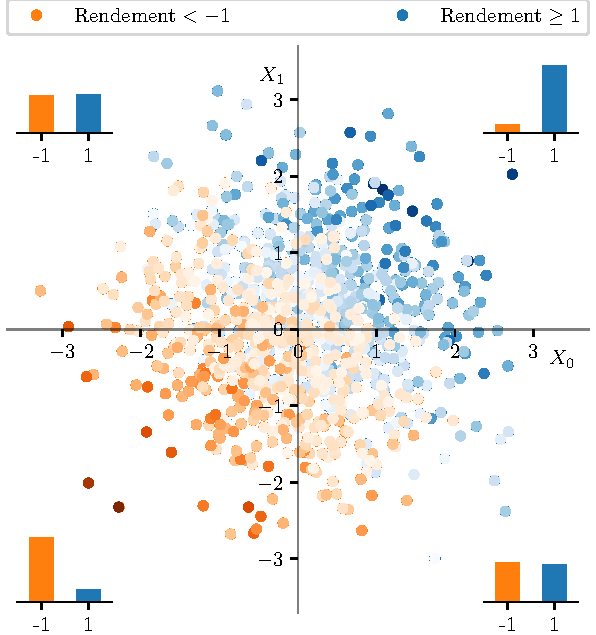
\includegraphics[width=\textwidth]{../experiments/fig/copula.pdf}
  \caption[Loi de marché]{Loi de marché théorique pour $\bar p = 2$. Les points bleus et
    rouges indiquent 500 réalisations d'une loi normale multivariée avec matrice de
    corrélation $\Sigma$. Les lois marginales Rademacher de la loi de marché entraînent un
    ``effondrement'' des réalisations en $\breve{X}_0$, $\breve{X}_1$ et $\breve{R}$ à
    leur signe. Les quatre histogrames présentent la distribution de $R$ par rapport à
    $X_0=\pm1$ et $X_1=\pm1$. On constate par ailleurs l'absence d'arbitrage d'une telle
    loi de marché puisqu'aucune région ne contient uniquement des rendements positifs ou
    uniquement des rendements négatifs.}
  \label{fig_copula}
\end{figure}


\begin{figure}[ht]
  \centering
  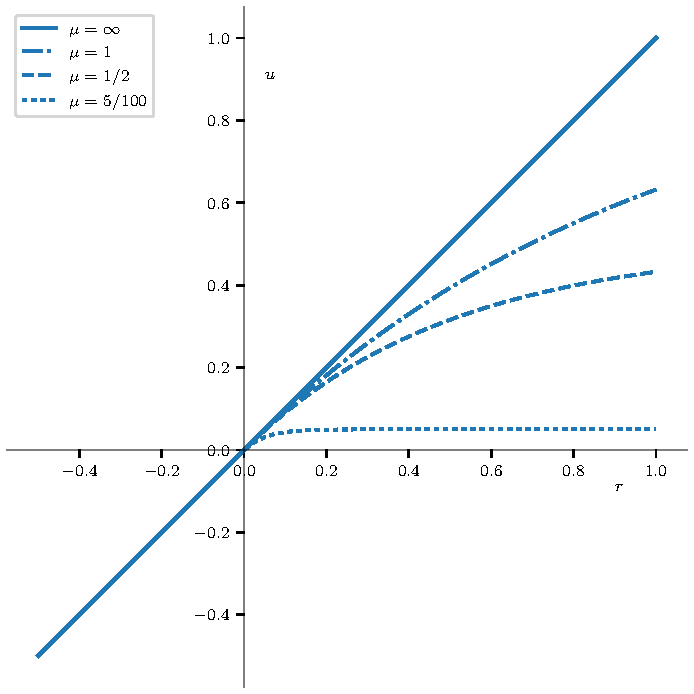
\includegraphics[width=\textwidth]{../experiments/fig/leus.pdf}
  \caption[Utilité Lipschitz exponentielle (LEU)]{Comportement des fonctions d'utilité
    exponentielles Lipschitz $\LEU_\mu$ selon le paramètre $\mu$. L'abscisse est l'axe des
    rendements, alors que l'ordonnée est celui des \textit{utils}. Le paramètre $\mu$ de
    chacune des instances $\LEU_\mu$ permet de quantifier l'aversion au risque : un
    paramètre $\mu\to\infty$ indique une attitude neutre au risque, alors qu'à l'autre extrême, un
    paramètre $\mu\to0$ modélise une indifférence (utilité constante) aux rendement
    positifs. Sur la branche négative, l'utilité correspond à la fonction identité, sur la
    branche positive, $\LEU_\mu(r) = \mu(1-e^{-r/\mu})$.}
  \label{fig_leus}
\end{figure}

\begin{figure}[ht]
  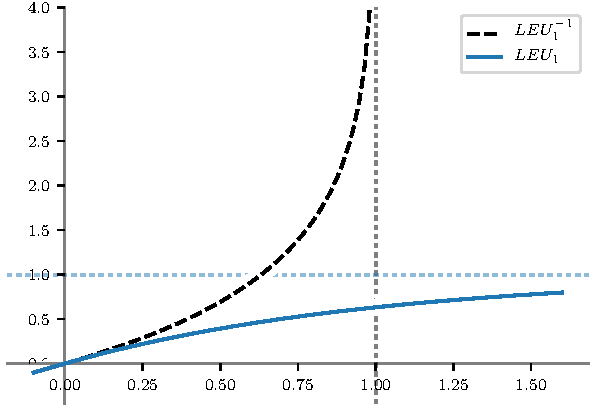
\includegraphics[width=\textwidth]{../experiments/fig/leu_inv.pdf}
  \caption[Fonction LEU et LEU inverse]{Utilité et utilité inverse. La fonction d'utilité
    permet de caractériser en \textit{utils} le rendement observé. L'\textit{util} est
    cependant une notion abstraite qu'on peut réexprimer en rendement à partir de la
    fonction utilité inverse. Une fonction $LEU_\mu(r)$ tend asymptotiquement vers $\mu$ à
    mesure que $r\to \infty$. Inversement, $LEU_\mu^{-1}(r)\to\infty$ à un rythme logarithmique lorsque
    $r\to\mu$. En effet, sur sa branche négative $\LEU_\mu^{-1}$ correspond à la fonction
    identité, alors que sur la branche négative, $\LEU_\mu^{-1}(r) = -\mu\log(1-r/\mu)$.}
  \label{fig_leu_inv}
\end{figure}

\clearpage


\subsection{\textit{n} variable, \textit{p} constant}
\label{emp:nvar}

L'objet de cette section est l'étude du cas canonique où la taille $n$ de l'ensemble
d'entraînement $\S_n$ augmente progressivement afin de donner une meilleure représentation
de $M$.


\subsubsection{Erreur de généralisation}

On rappelle tout d'abord que l'erreur de généralisation d'une politique d'investissement
$q$ consiste à mesurer la différence entre l'utilité (resp.~l'équivalent certain) espérée
observée en échantillon et l'utilité (resp.~l'équivalent certain) espérée hors
échantillon, ou, mathématiquement, de déterminer $\hEU(q) - \EU(q)$
(resp.~$\hCE(q) - \CE(q)$).

Avant de rentrer dans le vif du sujet, il peut être intéressant de voir graphiquement
comment se comportent différents quantiles de l'erreur de généralisation à mesure que de
nouveaux échantillons sont fournis à l'algorithme (\ie\ à mesure que $n$ augmente). La
Figure \ref{fig_genstats} illustre précisément ce comportement, en présentant l'erreur en
util et en rendement. Puisque la variable de rendement $R$ est bornée entre $-1$ et $1$ et
que son espérance marginale est nulle, le panneau b) indique qu'avec un échantillon
d'entraînement formé de $n=10$ observations de marché, l'erreur maximale sera d'environ
40\%. Par ailleurs, comme la courbe du 1\ier quartile correspond à une erreur nulle, on
peut conclure que dans environ 75\% des cas, la performance hors échantillon sera moindre
que celle observée en échantillon. Finalement, sans surprise, plus $n$ est élevé, moins
l'erreur de généralisation sera importante et tous ses quantiles finiront par converger
vers une erreur nulle. 


% La Table 1 indique par ailleurs le rythme de
% convergence des trois derniers quartiles d'erreur de généralisation en utilité. On
% constate que l'erreur médiane converge donc vers zéro presqu'à un rythme $\bigO(1/n)$
% alors que l'erreur maximale converge à un rythme près de $\bigO(n^{-1/2})$, donc plus
% lentement.


% \begin{table}[b]
%   \centering
%   \begin{tabular}{lSS[table-format = 1.3e1]}
%     \toprule
%     Quantile d'erreur & {Ordre de convergence} & \multicolumn{1}{c}{Erreur}\\
%     \midrule
%     Erreur maximale & -0.600 & 5.246e-03\\
%     75\ieme percentile d'erreur & -0.766 & 1.705e-03\\
%     Erreur médiane & -0.923 & 2.352e-03\\
%     \bottomrule
%   \end{tabular}
%   \caption{Ordre de convergence de chacun des trois derniers quartiles d'erreur de
%     généralisation (en util). L'erreur médiane converge donc vers zéro presqu'à un rythme
%     $\bigO(1/n)$ alors que l'erreur maximale converge à un rythme près de
%     $\bigO(n^{-1/2})$, donc plus lentement. Ce tableau a été produit à partir d'une
%     optimisation aux moindres carrés sur une fonction $an^k + b$, avec paramètres de
%     départ $b=0$, $a=1$ et $k=-1/2$.}
% \end{table}

La Figure \ref{fig_avrisk_gen} illustre quant à elle la relation entre l'aversion au
risque (caractérisée par le paramètre $\mu$ de la fonction d'utilité $\LEU$) et le 95\ieme
percentile d'erreur de généralisation en util et en équivalent certain. On constate en
particulier qu'une faible aversion au risque, toutes choses étant égales par ailleurs,
entraîne une plus grande erreur de généralisation. On peut expliquer cette observation
d'un point de vue géométrique, puisqu'une aversion plus prononcée au risque vient ajouter
de la courbure à la fonction d'utilité, et qu'en ce sens, cette courbure a le même effet
que l'ajout d'un terme de régularisation $\lambda\|q\|^2$ dans la fonction objectif de
l'algorithme. Or, comme l'idée même de la régularisation est de permettre d'établir des
politiques d'investissement plus conservatrices qui favorisent des investissement moins
importants, on comprend donc qu'une aversion au risque élevée aura le même genre d'effet
et entraînera donc une erreur hors échantillon moins importantes.

À la Figure \ref{fig_bound_errgen}, c'est le 95\ieme percentile d'erreur et sa borne
théorique $(\delta = 5\%)$ en fonction de $n$ qui sont illustrés, ce qui permet donc de
constater la pertinence des garanties théoriques offertes par l'algorithme
d'investissement. Ce qui frappe le plus, c'est surtout que la borne n'est pas exactement
serrée, les deux courbes différant l'une de l'autre d'un ordre de grandeur (soit d'un
facteur d'environ 10). Par exemple, il faut attendre d'avoir environ $n=150$ observations
avant de pouvoir garantir une erreur inférieure à 100\%, alors que le 95\ieme percentile
d'erreur empirique n'y est que de 5\%.

Néanmoins, il faut d'abord conserver à l'idée que ces bornes sont valides pour toute loi
de marché $M$ telle que $\xi\leq\sqrt{2}$ et $\rmax\leq 1$ et toute courbe d'utilité $u$ de
coefficient Lipschitz 1. C'est toutefois avec cette forme particulière de $M$ (marges
Rademacher) qu'on a pu observer les bornes plus serrées. Mais d'autre part, si les bornes
ne sont en tant que telles pas particulièrement fortes, l'ordre $\bigO(n^{-1/2})$ qu'elles
indiquent semble bien respecté empiriquement. Cette propriété est très importante
puisqu'elle permet à un investisseur de savoir de quelle façon et à quel rythme décroît
son risque d'erreur de généralisation en fonction de la taille de son ensemble
d'entraînement $\S_n$. 

Il peut en outre être intéressant de décomposer ce 95\ieme percentile d'erreur de
généralisation en sa composante de performance en échantillon $\hEU(\qh)$ et hors
échantillon $\EU(\qh)$ (Figure \ref{fig_bound_gencomps}). Cette figure permet de constater
que bien que la composante hors échantillon possède une utilité espérée positive, elle
sera cependant beaucoup plus faible que ce qui était anticipé par l'utilité espérée en
échantillon. De plus, la composante hors échantillon demeure relativement stable et c'est
la composante en échantillon qui converge vers elle. De plus, cette figure permet de
comprendre comment on peut passer d'une représentation en util à une représentation en
rendement suite à l'application de la fonction utilité inverse $\LEU^{-1}_\mu:\Ut \to \R$
(voir Figure \ref{fig_leu_inv}). Puisque $\mu=1$ ici, cette utilité inverse a un effet plus
prononcé pour des utilités proches de 1, et son effet décroit pour des utilités plus
faibles. Bien entendu, cette amplification est plus prononcée à mesure que l'investisseur
est averse au risque, ce qui dégrade alors la qualité des garanties offertes par
l'algorithme.


\newpage


\begin{figure}[h!]
  \centering
  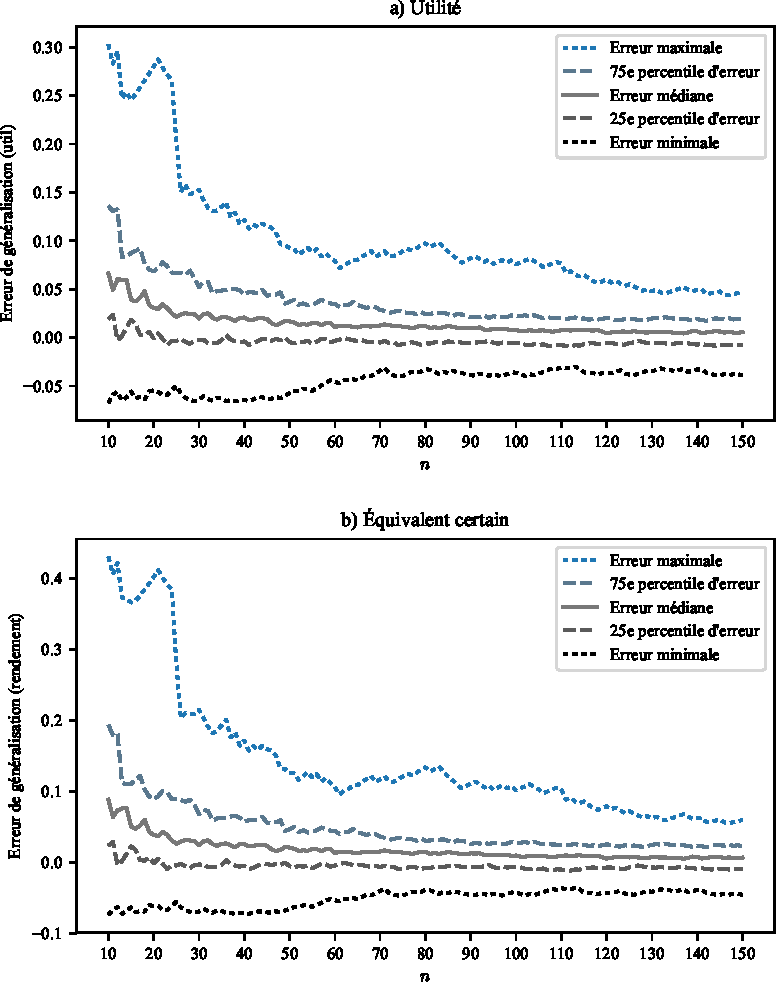
\includegraphics[width=\textwidth]{../experiments/fig/genstats.pdf}
  \caption[Quartiles de l'erreur de généralisation]{Progression des quartiles de l'erreur
    de généralisation en util et en équivalent certain en fonction de la taille $n$ de
    l'échantillonage. Dans environ 75\% des cas, la performance hors échantillon sera
    moindre que celle observée en échantillon. }
  \label{fig_genstats}
\end{figure}


\begin{figure}[h!]
  \centering
  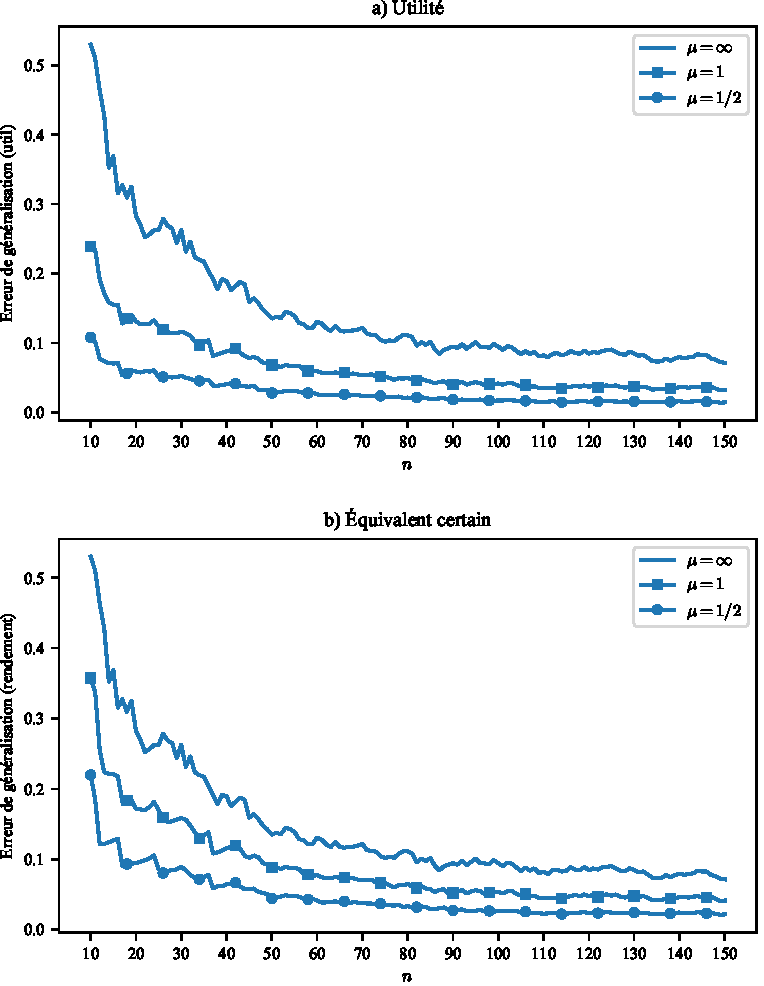
\includegraphics[width=\textwidth]{../experiments/fig/avrisk_gen.pdf}
  \caption[Aversion au risque et erreur de généralisation]{Progression du 95\ieme
    percentile d'erreur de généralisation en fonction de la taille de l'échantillon $n$
    pour trois niveaux d'aversion au risque. Plus l'aversion au risque est faible (avec
    comme cas limite l'attitude neutre au risque $\mu = \infty$), plus l'erreur de généralisation
    est importante, et inversement pour une forte aversion au risque. }
  \label{fig_avrisk_gen}
\end{figure}



\begin{figure}[h!]
  \centering
  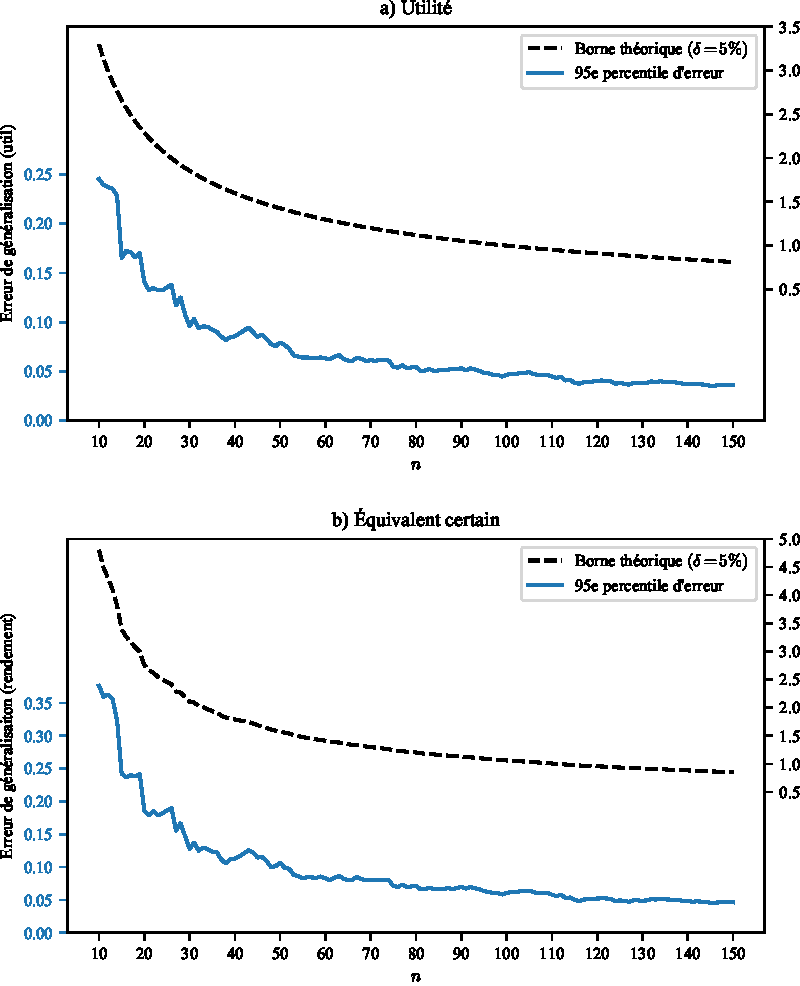
\includegraphics[width=\textwidth]{../experiments/fig/bound_errgen.pdf}
  \caption[Erreur de généralisation en fonction de $n$]{Progression du 95\ieme
    percentile l'erreur de généralisation et borne théorique (paramètre de confiance
    $\delta = 5\%$) en fonction de la taille d'échantillon $n$, exprimés en util et en
    rendement. Dû à la différence d'ordre, les deux figures font intervenir deux
    ordonnées: celle de gauche quantifie l'erreur empirique alors que celle de droite
    quantifie la borne théorique. Ainsi, la borne théorique est environ 10 fois supérieure
    à l'erreur empirique.}
  \label{fig_bound_errgen}
\end{figure}

\begin{figure}[h!]
  \centering
  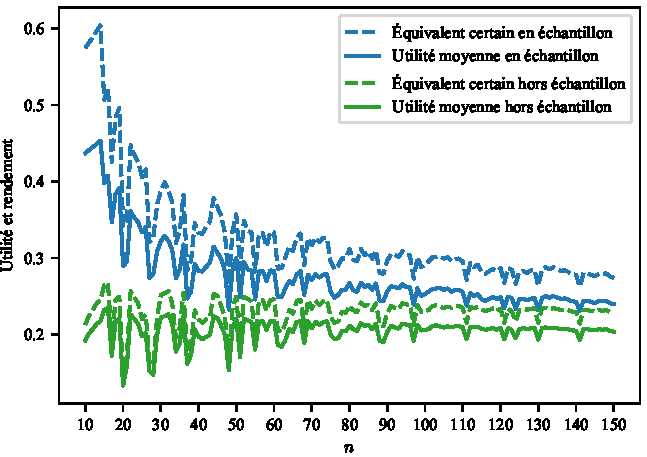
\includegraphics[width=\textwidth]{../experiments/fig/bound_gencomps.pdf}
  \caption[Composantes de l'erreur maximale]{Progression sur la même échelle des
    composantes de performance en échantillon et hors échantillon, exprimées en util et en
    rendement, du 95\ieme percentile d'erreur de généralisation de la Figure
    \ref{fig_bound_errgen} a). Plus une valeur d'utilité est grande, plus l'amplification
    de l'utilité inverse se fera ressentir. L'erreur de généralisation est donc plus
    importante lorsqu'elle est mesurée en unités de rendement qu'en unités d'utils.  }
  \label{fig_bound_gencomps}
\end{figure}

\clearpage


\subsubsection{Erreur de sous optimalité}

Contrairement à l'erreur de généralisation, l'erreur (en util) de sous optimalité
$\EU(\qs) - \EU(\qh)$ (resp.~$\CE(\qs) - \CE(\qh)$ dans le domaine des rendements) ne
bénéficie pas d'une convergence vers zéro du fait de la présence du terme de
régularisation dans l'algorithme $\alg(\S_n)$. En fait, la meilleure garantie offerte par
le Théorème \ref{thm3}, lorsque $n\to\infty$, correspond à $\lambda/2\|\qs\|^2$ dans le domaine des
utils.

Ainsi, la Figure \ref{fig_bound_errso} présente la progression du 95\ieme percentile de
l'erreur empirique de sous optimalité et de la borne théorique $\delta = 5\%$ selon la taille
$n$ de l'échantillon. En particulier, le facteur de régularisation constant $\lambda = 1$ fait
en sorte que, exprimés en utils, la borne théorique converge vers $\|q^\star\|^2/2$ (évaluée
numériquement à \num{3.16}) alors que le 95\ieme percentile d'erreur semble converger vers
une utilité espérée aux alentours de \num{0.24}.

D'autre part, la borne théorique de sous optimalité du 95\ieme percentile d'erreur
empirique est relâchée d'environ deux ordres de grandeur ($10^{-1}$ pour l'erreur
empirique \textit{vs} $10^{2}$ pour la garantie théorique). En fait, ce qui est
particulièrement déconcertant, c'est que même dans la limite $n\to\infty$, la borne théorique est
supérieure à la plus grande erreur empirique observée (\ie\ lorsque $n=10$)!  Cela étant,
même si la borne de sous optimalité est particulièrement relâchée, elle suggère en
revanche un ordre de convergence $\bigO(n^{-1/2})$ qui lui semble être en adéquation avec
le 95\ieme percentile de l'erreur de sous optimalité empirique.

Néanmoins, un investisseur ayant à cœur une faible erreur de sous optimalité devra
nécessairement faire converger son paramètre de régularisation vers zéro à mesure que de
nouvelles observations de la loi de marché sont disponibles. De plus, il a été démontré au
cours de la section précédente qu'on doit avoir $\lambda = \omega(1/\sqrt{n})$, \ie\ une décroissance
moins rapide que $\bigO(1/\sqrt{n})$ pour bénéficier d'une convergence vers une erreur
nulle. En particulier, si $\lambda = \bigO(n^{-k})$, alors la garantie théorique sera composée
de trois termes : $\bigO(n^{k-1}) + \bigO(n^{k-1/2}) + \bigO(n^{-k})$. Dans de telles
conditions, une constante $k=1/4$ semble bien adaptée pour balancer les deux derniers
termes.

Ainsi, la Figure \ref{fig_bound_errso3} présente la progression du 95\ieme percentile
d'erreur de sous optimalité empirique et de sa garantie théorique en fonction de $n$
lorsque $\lambda=(10/n)^{1/4}$. Ainsi défini, lorsque $n=10$, $\lambda$ est identique au facteur de
régularisation employé pour produire la Figure \ref{fig_bound_errso}. On constate
effectivement que l'erreur de sous optimalité est initialement la même pour les deux
figures. Cependant, alors qu'elle paraîssait stagner vers une erreur de 34\% avec une
régularisation constante, la décroissance $\lambda = \bigO(n^{-1/4})$ permet ici d'obtenir une
erreur de 26\% lorsque $n=150$. Par contre, il faut être bien conscient que la borne
théorique ne décroît plus qu'à un rythme $\bigO(n^{1/4})$.

\newpage

\begin{figure}[h!]
  \centering
  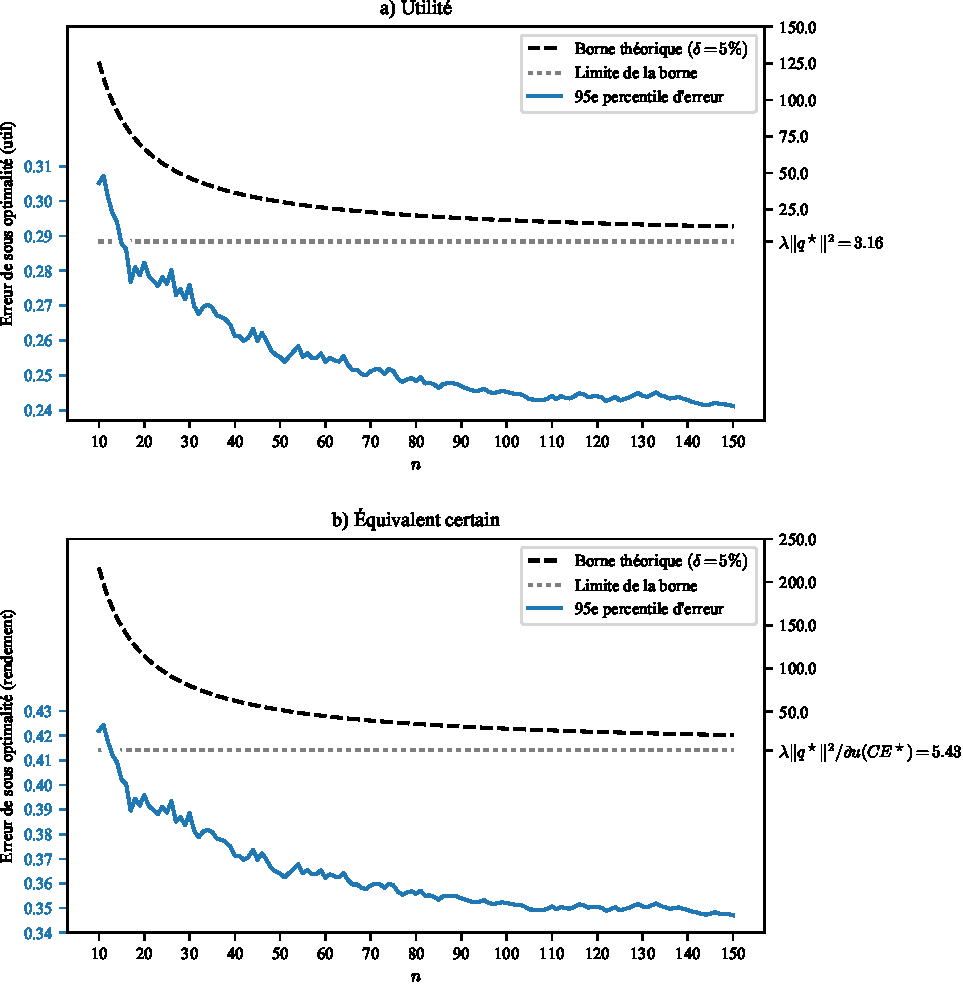
\includegraphics[width=1.3\textwidth]{../experiments/fig/bound_errso.pdf}
  \caption[Erreur de sous optimalité en fonction de $n$ ($\lambda$
  constant)]{Progression du 95\ieme percentile l'erreur empirique de sous optimalité et de
    la borne théorique $(\delta = 5\%)$ selon la taille $n$ de l'échantillonage. Le facteur de
    régularisation constant $\lambda = 1$ fait en sorte que, exprimés en utils, la borne
    théorique planche à $\lambda/2\|q^\star\|^2$ (évaluée numériquement à \num{3.16}) alors que le
    95\ieme percentile d'erreur semble plancher aux alentours de \num{0.24}. En plus
    d'être dégagée de près d'un ordre de grandeur de la courbe empirique, même la limite
    de la borne théorique est supérieure aux plus hautes valeurs observées. Cependant,
    l'ordre $\bigO(n^{-1/2})$ théorique se manifeste ici aussi dans le domaine empirique.}
  \label{fig_bound_errso}
\end{figure}

\begin{figure}[h!]
  \centering 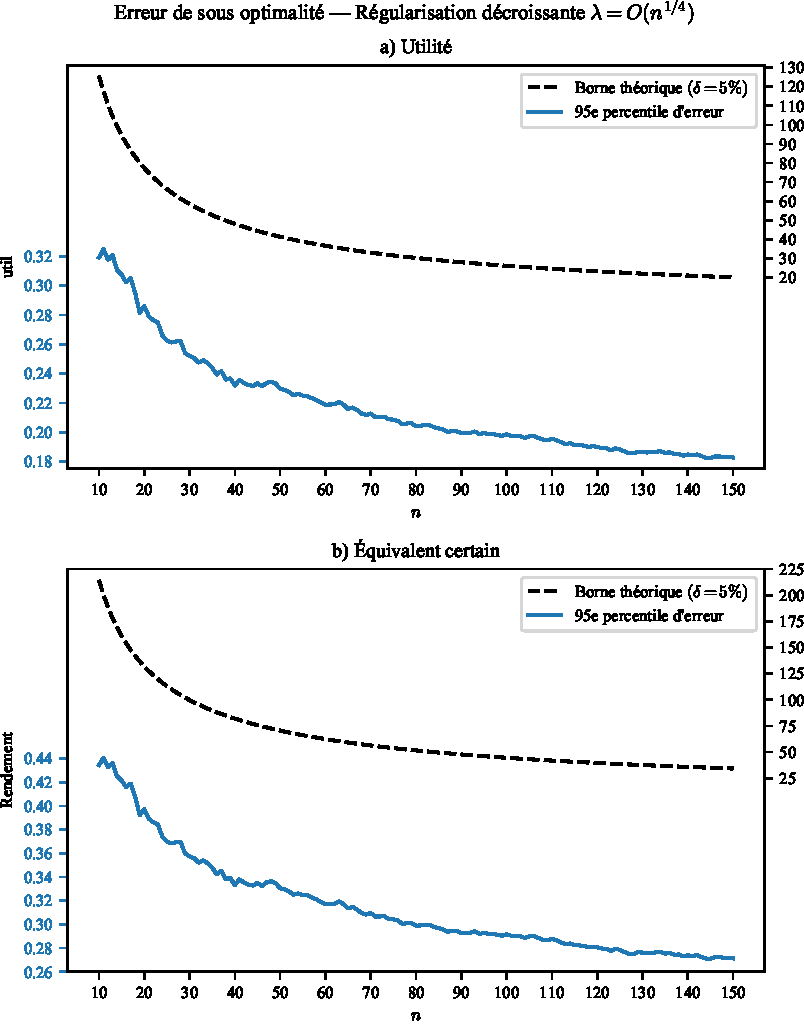
\includegraphics[width=\textwidth]{../experiments/fig/bound_errso3.pdf}
  \caption[Erreur de sous optimalité en fonction de $n$
  ($\lambda=\bigO(n^{-1/4})$)]{Progression du 95\ieme percentile de l'erreur de sous optimalité
    empirique exprimée en util et de la borne théorique $\delta=5\%$ selon la taille $n$ de
    l'échantillonage avec un facteur de régularisation $\lambda = (10/n)^{1/4}$. Le panneau a)
    indique la progression de la borne théorique alors que le panneau b) indique sa limite
    de la borne dans le cas $n\to\infty$. Contrairement au cas présenté à la Figure
    \ref{fig_bound_errso}, cette situation offre une garantie théorique d'une erreur nulle
    puisque le facteur de régularisation converge vers 0. Le rythme de convergence
    théorique n'est toutefois que de $\bigO(n^{-1/4})$.}
  \label{fig_bound_errso3}
\end{figure}


\clearpage

\subsection{\textit{n} constant, \textit{p} variable}
\label{emp:pvar}

Cette section sera consacrée à l'étude du rapport qu'entretient les erreurs de
généralisation et de sous-optimalité de notre algorithme lorsque sont incorporées à la
prise de décision de nouvelles variables de marché indépendantes des précédantes, tout en
conservant la taille d'échantillonnage constante.

On rappelle donc que les expériences suivantes dévoileront une à une les 50 variables de
marché $X_j$ à partir desquelles le rendement aléatoire $R$ est construit sur une copule
gaussienne. Trois situations différentes seront par ailleurs considérées, chacune d'elles
représentée respectivement par les vecteurs de corrélation
$\Corr(\tilde X,\tilde R) \in \Re^{\bar p}$ (dans le domaine de la copule gaussienne)
suivants:
\begin{gather}
  \rho = \left(\begin{matrix}\sqrt{\frac{1-\epsilon}{\bar p}} & \cdots & \sqrt{\frac{1-\epsilon}{\bar
          p}}\end{matrix}\right)\,;\\
  \rho = \left(\begin{matrix}\sqrt{1-\epsilon} & 0 & \cdots & 0\end{matrix}\right)\,;\\
  \rho = \left(\begin{matrix}0 & \cdots & 0\end{matrix}\right).
\end{gather}

La première situation sera donc celle où chacune des variables de marché a une influence
égale sur le rendement, la seconde celle où seule la première variable vient influencer la
réalisation du rendement et enfin la dernière celle où toutes les variables de marché sont
indépendantes au rendement, \ie\ elle ne forment qu'un ``bruit''. Ces trois situations
seront désignées respectivement par \textit{information dispersée}, \textit{information
  concentrée} et \textit{aucune information}.


\subsubsection{Erreur de généralisation}


La figure \ref{fig_pconst_infogen} présente donc pour ces trois situations comment
progresse leur 95\ieme percentile d'erreur de généralisation (avec $\bar n = 10$
observations du marché) et leur garantie théorique (ici commune aux trois cas) à mesure
que de nouvelles variables de marché sont dévoilées à l'algorithme. Intialement, lorsque
$p=1$ , la courbe \textit{Information concentrée} affiche sans surprise une erreur
beaucoup plus faible que les autres, puisque l'algorithme est déjà en mesure d'inférer la
meilleure politique d'investissement. Au contraire, la courbe \textit{Information
  dispersée} ne détecte qu'un faible lien entre cette variable de marché et $R$. À mesure
que de nouvelles varialbes sont dévoilée, la situation où l'information concentrée
continue de présenter une erreur plus faible aux autres cas, bien que la courbe d'erreur
dans la courbe \textit{Information dispersée} semble finir par la rejoindre. C'est de plus
lorsqu'aucune information n'est présente que le risque d'erreur de généralisation est le
plus grand, puisque toute décision d'investissement non nulle se traduit forcément par une
utilité hors échantillon plus faible qu'en échantillon.

En outre, la garantie sur l'erreur de généralisation, dans le cas d'un apprentissage par
noyau linéaire et d'une taille constante d'échantillonnage, suggère une progression de
l'erreur à un rythme linéaire $\bigO(p)$ (voir Section \ref{b:dim}). Or, les trois courbes
d'erreur empirique semblent indiquer qu'il se pourrait que ce ne soit que le cas que dans
une limite asymptotique, non observée dans ce cas ci. En effet, leur forme est loin d'être
linéaire et semble plutôt posséder une composante racine carrée. Il se pourrait donc que
le comportement de l'erreur de généralisation soit plutôt de $\bigO(p^{1/2}) + \bigO(p)$.

Afin de confirmer cette idée, la figure \ref{fig_pconst_infogen_cf} présente un ajustement
des 25 derniers points des trois courbes d'erreurs empiriques à deux fonctions
polynômiales $f(x) = a_0x + a_1x^{1/2} + b$ et $f(x) = a_0x^{1/2} + b$ par méthode des
moindres carrés. Il faut garder à l'esprit qu'estimer numériquement un ordre polynômial
n'est pas forcément simple, particulièrement lorsqu'on ne dispose que de si peu de points
($\bar p = 50$ dans ce cas-ci). Cela dit, dans les trois cas, l'hypothèse où l'erreur de
généralisation serait de nature $\bigO(p^{1/2}) + \bigO(p)$ semble plus convaincante
puisqu'elle suit de plus proche les vingt cinq premiers points des trois courbes. Cette
conclusion reste cependant spéculative.

\subsubsection{Sous optimalité}

Dans le cas où on ajoute de l'information, la sous optimalité, contrairement à l'erreur de
généralisation, peut référer à deux types d'erreur. Soit on compare la performance hors
échantillon de $\qh$ à celle de la politique optimale qui ne dispose que de
$p \leq \bar p$ variables d'information, soit à la politique optimale qui dispose des
$\bar p$ variables d'information nécessaires pour décrire $M$. Cependant, le développement
théorique qui a été mené au cours de la dernière section ne s'est implicitement préoccupé
que de la première situation.

La Figure \ref{fig_pconst_euinforelative} indique le comportement de l'utilité espérée
optimale $\nEU^\star$ en fonction du nombre de variables de marché connues de
l'algorithme. Naturellement, le cas où toute l'information est disponible dès $p=1$
affiche une utilité espérée optimale constante, alors qu'il s'agit plutôt d'une
progression à peu près linéaire lorsqu'on dévoile progressivement des variables
d'information chacunes faiblement corrélées à $R$, mais indépendantes l'une à
l'autre. Enfin, l'utilité espérée optimale est bien entendu nulle dans le cas où toutes
les variables de marché sont indépendantes à $R$.

La Figure \ref{fig_pconst_infosorelative} elle, indique la progression du 95\ieme
percentile des erreurs de sous optimalité des trois situations et de leur garantie
théorique pour $\delta = 5\%$ à mesure que de nouvelles variables de marché sont dévoilées à
l'algorithme, avec $\bar n = 10$ constant. Initialement, l'erreur de sous optimalité des
courbes \textit{Information dispersée} et \textit{Aucune information} est très faible
alors que la courbe \textit{Information concentrée} dispose déjà de suffisament
d'information pour permettre une erreur élevée. Puis, à mesure que $p$ se rapproche de
$\bar p$, on observe pour la courbe \textit{Information dispersée} une progression qui
correspond environ à la progression de l'utilité espérée optimale. Cela signifie donc que
l'erreur de sous optimalité serait maximisée lorsque l'utilité espérée hors échantillon
est nulle. Les deux autres courbes d'erreur empirique progressent beaucoup plus lentement,
possiblement à un rythme $\bigO(\sqrt{p})$. Dans le cas de la courbe \textit{Information
  concentrée}, puisque sa courbe de référence $\nEU^\star$ est constante, on en conclut
que l'utilité espérée hors échantillon minimale augmente selon $\bigO(\sqrt{p})$. 

De plus, le caractère linéaire annoncé n'est empiriquement pas très clair, sauf dans le
cas particulier où l'information est dispersée. Mais comme c'état le cas pour l'erreur de
généralisation, il n'est pas non plus impossible que l'erreur de sous optimalité ait un
ordre de progression $\bigO(\sqrt{p}) + \bigO(p)$: cela permettrait d'expliquer pourquoi
la courbe \textit{Information dispersée} est linéaire alors que les deux autres affichent
plutôt un caractère de progression racine carrée.
\newpage

\begin{figure}[h!]
  \centering
  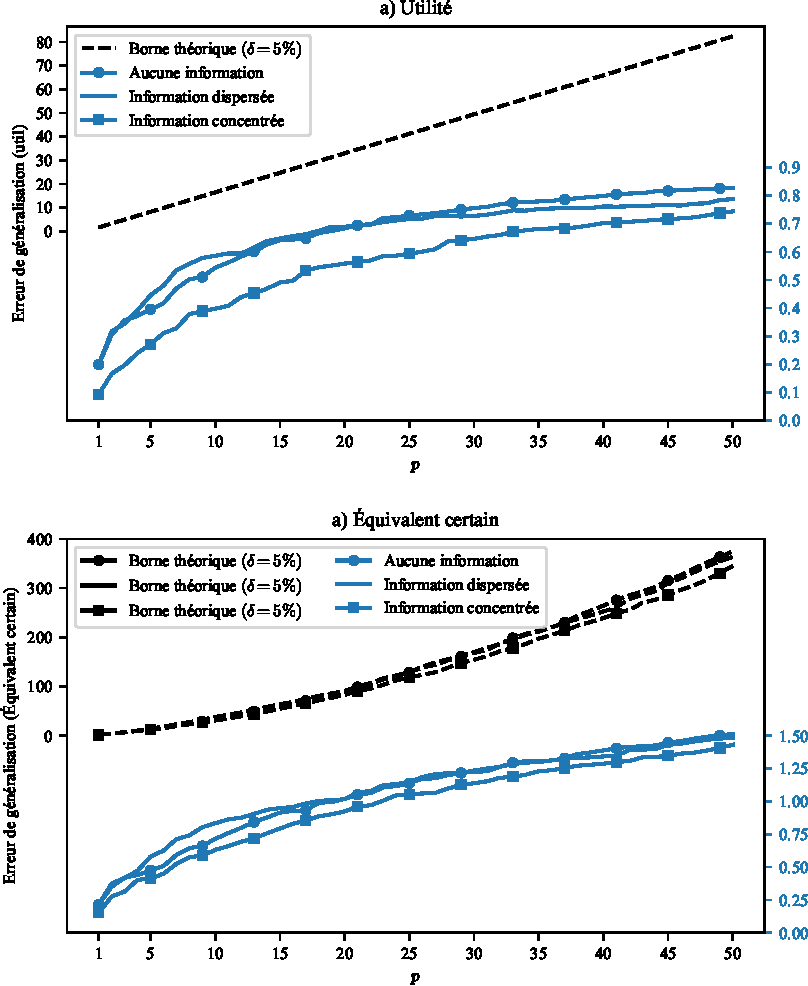
\includegraphics[width=1\textwidth]{../experiments/fig/pconst_infogen2.pdf}
  \caption[Erreur de généralisation en fonction de $p$]{Progression du 95\ieme percentile
    de l'erreur de généralisation exprimée en util et en équivalent certain à mesure que
    de nouvelles variables de marché sont dévoilées à l'algorithme, pour une taille
    d'échantillonnage constante $\bar n = 10$. Dans le domaine des utils, illustré par le
    panneau a), la borne théorique est commune aux trois situations et progresse
    linéairement. Lorsque $p=1$, la courbe \textit{Information concentrée} affiche sans
    surprise une erreur initialement plus faible que les autres, puisque l'algorithme est
    déjà en mesure d'inférer la meilleure politique d'investissement. Les courbes
    \textit{Aucune information} et \textit{Information dispersée} présentent une erreur
    similaire lorsque $p$ est faible (donc peu de variables connues) mais se distancent
    l'une de l'autre à mesure que $p$ converge vers $\bar p$.}
  \label{fig_pconst_infogen}
\end{figure}

\begin{figure}[h!]
  \centering
  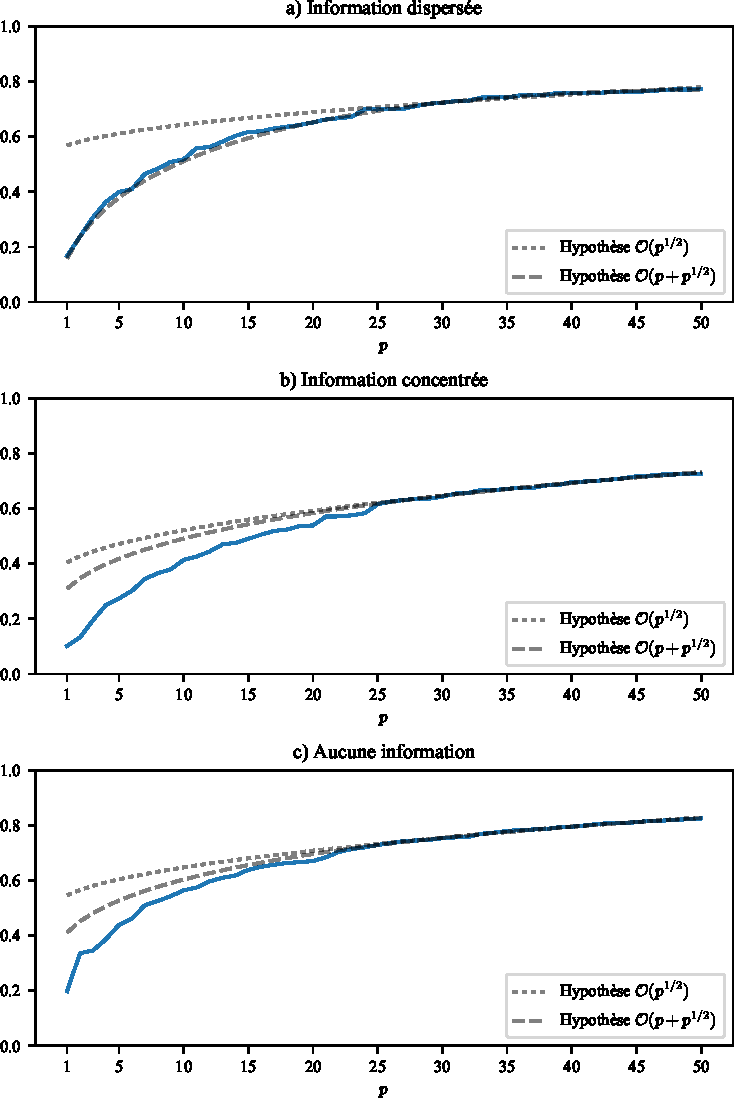
\includegraphics[width=1\textwidth]{../experiments/fig/pconst_infogen_cf.pdf}
  \caption[Ajustement des courbes d'erreurs de généralisation]{Ajustement des 25 derniers
    points des courbes d'erreur présentées à la Figure \ref{fig_pconst_infogen} à deux
    polynômes $f(p) = a_0p + a_1 p^{1/2} + b$ et $f(p) = a_0p + b$. Entre les deux,
    l'hypothèse où l'erreur aurait une progression $\bigO(p^{1/2}) + \bigO(p)$ serait
    ainsi la plus probable.}
  \label{fig_pconst_infogen_cf}
\end{figure}

\clearpage




\begin{figure}[h!]
  \centering
  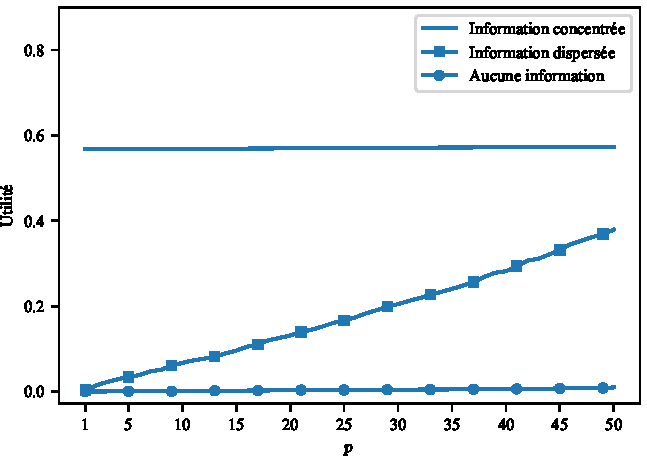
\includegraphics[width=\textwidth]{../experiments/fig/pconst_euinforelative.pdf}
  \caption[Utilité espérée optimale en fonction de $p$]{Progression de l'utilité espérée
    optimale $\nEU^\star$ en fonction du nombre de variables de marché connues. Naturellement,
    le cas où toute l'information est disponible dès $p=1$ affiche une utilité espérée
    optimale constante, alors qu'il s'agit plutôt d'une progression à peu près linéaire
    lorsqu'on dévoile progressivement des variables d'information chacunes faiblement
    corrélées à $R$, mais indépendantes l'une à l'autre. Enfin, l'utilité espérée optimale
    est bien entendu nulle dans le cas où toutes les variables de marché sont
    indépendantes à $R$. Les bornes théoriques exprimées en util se confondent car elles
    sont numériquement très rapprochées.}
  \label{fig_pconst_euinforelative}
\end{figure}

\begin{figure}[h!]
  \centering
  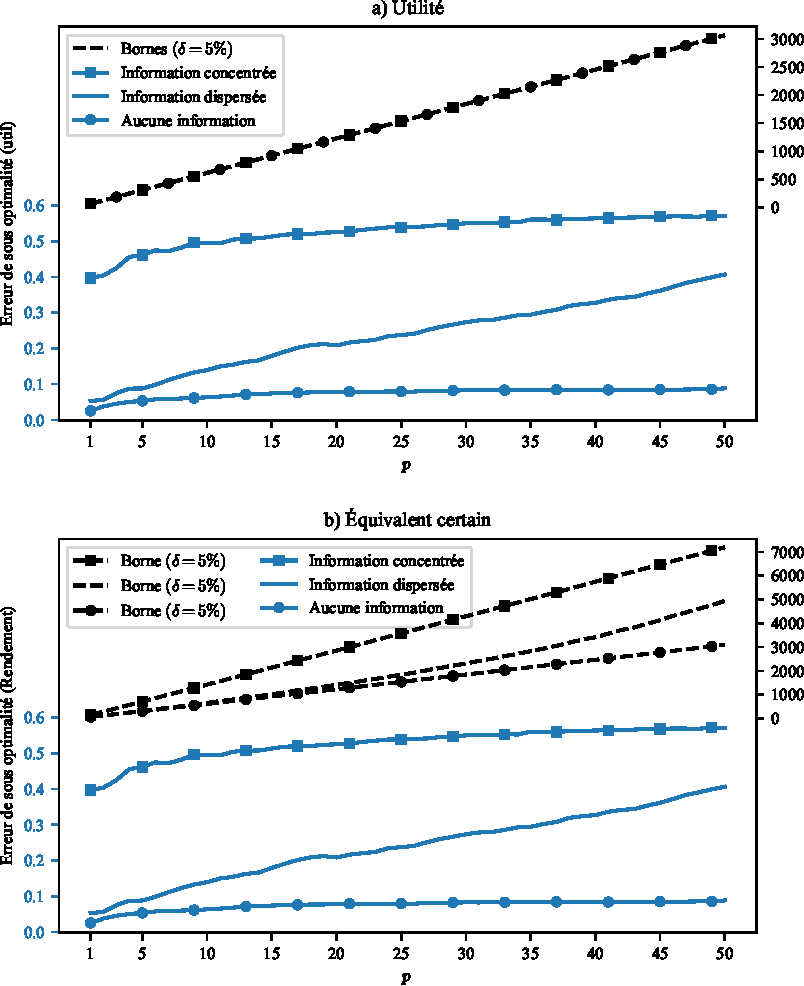
\includegraphics[width=\textwidth]{../experiments/fig/pconst_so.pdf}
  \caption[Erreur de sous optimalité en fonction de $p$]{Progression du 95\ieme percentile
    des erreurs de sous optimalité et de leur garantie théorique à mesure que de nouvelles
    variables de marché sont dévoilées à l'algorithme, avec $\bar n = 10$
    constant. Initialement, l'erreur de sous optimalité des courbes \textit{Information
      dispersée} et \textit{Aucune information} est très faible alors que la courbe
    \textit{Information concentrée} dispose déjà de suffisament d'information pour
    permettre une erreur élevée. Puis, à mesure que $p$ se rapproche de $\bar p$, on
    observe pour la courbe \textit{Information dispersée} une progression linéaire, alors
    que l'erreur plafonne dans les deux autres cas. Les garanties en util donnent une
    progression qui elle est linéaire en util. }
  \label{fig_pconst_infosorelative}
\end{figure}


\clearpage

\subsection{\textit{n} et \textit{p} variables}
\label{emp:npvar}

Finalement, cette section cherche à illustrer le comportement de l'erreur de
généralisation et de sous optimalité lorsqu'on est en présence de régimes dynamiques entre
$n$ et en $p$, \ie\ lorsque $p=\bigO(n^k)$. Trois régimes seront étudiés : celui où
$p=\bigO(n^{1/2})$, $p=\bigO(n^{3/4})$ et $p=\bigO(n)$. La façon de procéder restera la
même que celle employée aux sections précédentes. Les percentiles d'erreur seront
déterminés à partir d'un échantillon formé de $m=150$ ensembles d'entraînement de taille
$n$, $n$ variant de 9 à 50. Le nombre de variables de marché dévoilées sera ensuite donné
à partir d'une des trois relations suivantes : $p=2n$, $p=3.5n^{3/4}$ et $p=6n^{1/2}$,
selon le régime. Le marché sera constitué de $\bar p = 100$ variables, ce qui correspond à
$p(\bar n)$ dans le régime $p = \bigO(n)$. Ces relations ont été déterminées afin que les
valeurs initiales de $p$ soient identiques et qu'elles conservent le même ordre de
grandeur sur toute l'expérience (voir Figure \ref{fig_np_np}).

\begin{figure}[h]
  \centering
  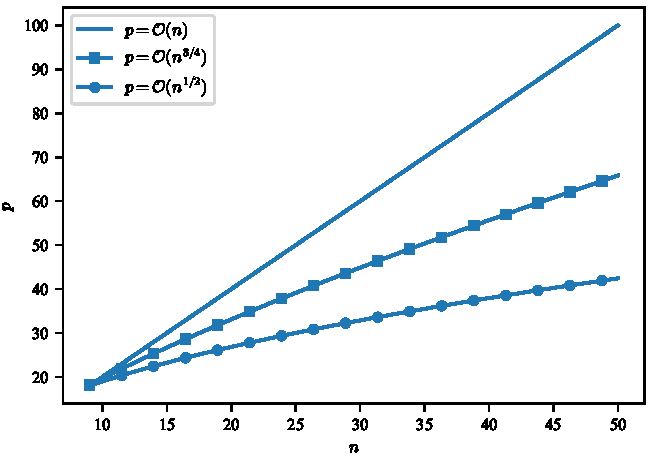
\includegraphics[width=0.7\textwidth]{../experiments/fig/np_np.pdf}
  \caption[Progression des trois régimes $p=\bigO(n^{1/2}),\bigO(n^{3/4}),\bigO(n)$]{En
    fonction de $n$, trois de cas de figure seront étudiés où le nombre $p$ de variables
    de marché dévoilées à l'algorithme dépend de $n$. Dans les expériences de cette
    section, $n$ variera de $9$ à $50$. La relation entre $p$ et $n$ sera alors
    respectivement donnée par $p = 2n$, $p=3.5n^{3/4}$ et $p=6n^{1/2}$.}
  \label{fig_np_np}
\end{figure}


Les propriétés mathématiques des deux types d'erreur établies à la Section \ref{b:dim}
suggérait un ordre asymptotique $\bigO(p\,n^{-1/2})$. Les résultats empiriques de la Section
\ref{emp:nvar} (\textit{n} variable, \textit{p} constant) ont d'abord permis de confirmer
l'ordre $\bigO(1/\sqrt{n})$ avec $p$ constant. Puis à la Section \ref{emp:pvar}
(\textit{n} constant, \textit{p} variable), la progression qu'on aurait pu anticiper être
linéaire s'est révélée comporter possiblement une composante racine carrée, \ie\
$\bigO(p) + \bigO(\sqrt{p})$. Ainsi, uniquement à partir de ces observations, on pourrait
conjecturer que l'erreur se comporte en fait comme
$\bigO(p/\sqrt{n}) + \bigO(\sqrt{p/n})$. Du fait de la dominance de $1/\sqrt{n}$ sur
$1/n$, rien n'empêcherait non plus que l'ordre soit $\bigO(p/n) + \bigO(\sqrt{p/n})$.


\subsubsection{Erreur de généralisation}


La Figure \ref{fig_bound_npgenu} présente la progression du 95\ieme percentile de l'erreur
de généralisation et de la garantie théorique ($\delta = 5\%$) des trois régimes de $p$ en
fonction de la taille d'échantillonage $n$. Ce qui frappe surtout, c'est comment les
ordres théoriques n'ont rien à voir avec les ordres empiriques. Soit par exemple le cas où
$p=\bigO(\sqrt{n})$. La courbe de la garantie demeure constante alors qu'en fait c'est
plutôt une décroissance qui est observée. Si on a plutôt une progression $p=\bigO(n)$, il
aurait été raisonnable de penser que l'erreur de généralisation augmenterait, alors que
même dans ce cas, elle continue de décroître!

La Figure \ref{fig_np_np32} présente le 95\ieme percentile de l'erreur de généralisation
suivant un autre régime où $p=0.0016n^{3/2}$. Si l'erreur est alors bien croissante, il
faut être prudent et éviter de généraliser cette observation puisque la valeur de départ
$p = 1$ lorsque $n=9$ n'est pas la même que pour les trois régimes de la Figure
\ref{fig_bound_npgenu} où $p=18$ lorsque $n=9$. Mais de toute façon, les résultats de la
Section \ref{emp:pvar} confirment qu'il existe un point où si $p$ domine suffisament $n$
l'erreur de généralisation devra croître. Il n'est cependant pas clair quel est ce point,
ni comment il dépend de $n$ ou de $p$.


\subsubsection{Erreur de sous optimalité}

La Figure \ref{fig_bound_npgsou} présente quant à elle la progression du 95\ieme
percentile de l'erreur de sous optimalité de la borne de généralisation selon les trois
régimes à l'étude, $p=\bigO(n^{1/2}),p=\bigO(n^{3/4})$ et $p=\bigO(n)$. L'ordre
$\bigO(p/\sqrt{n})$ de la borne théorique semble ici respecté, puisque l'erreur de sous
optimalité demeure constante dans le cas $p=\bigO(\sqrt{n})$, alors qu'elle augmente dans
les deux autres cas. Cependant, les courbes théoriques décroissent, excepté lorsque
$p=\bigO(n)$!

Pour expliquer ce phénomène contre intuitif, il suffit de réaliser que la borne théorique
a en fait une croissance $\bigO(p/\sqrt{n}) + \bigO(\sqrt{p/n}) + \bigO(1)$. Donc si
$p=\bigO(\sqrt{n})$, l'ordre asymptotique de l'erreur sera alors $\bigO(1)$, \ie\ constant
mais le deuxième terme forcera une décroissance $\bigO(\sqrt{n})$ vers cette constante, et
c'est précisément cette décroissance qu'on observe dans la Figure \ref{fig_bound_npgsou}.

De plus, il ne faut pas oublier que la norme de la décision optimale
$\lambda\|q^\star\|^2$ entre aussi dans la composition de la borne théorique, et donc possiblement
dans celle de l'erreur empirique de sous optimalité. Hélas, l'ordre de grandeur de cette
décision optimale est inconnue.

Cette figure illustre en fait assez bien le problème à réduire la progression des erreurs
en ordres asymptotiques. En effet, si l'erreur est polynômiale, alors même si un certain
ordre doit émerger asymptotiquement, lorsque $n$ est fini, il est tout à fait possible que
ce soit un terme d'un autre ordre qui domine la progression.  Avec les paramètres choisis
pour l'expérience de la Figure \ref{fig_bound_npgsou}, si l'ordre de l'erreur de sous
optimalité est effectivement de $\bigO(p/\sqrt{n}) + \bigO(\sqrt{p/n})$, alors il est
clair que seule la première composante joue sur la progression de l'erreur. À la Section
\ref{emp:pvar} où le cas où $n$ étant constant était étudié, il semblait pourtant que
l'erreur progresse en $\bigO(\sqrt{p}) + \bigO(p)$, ce qui laisse donc finalement assez
incertain l'ordre véritable de l'erreur de sous optimalité.


\begin{figure}[h!]
  \centering
  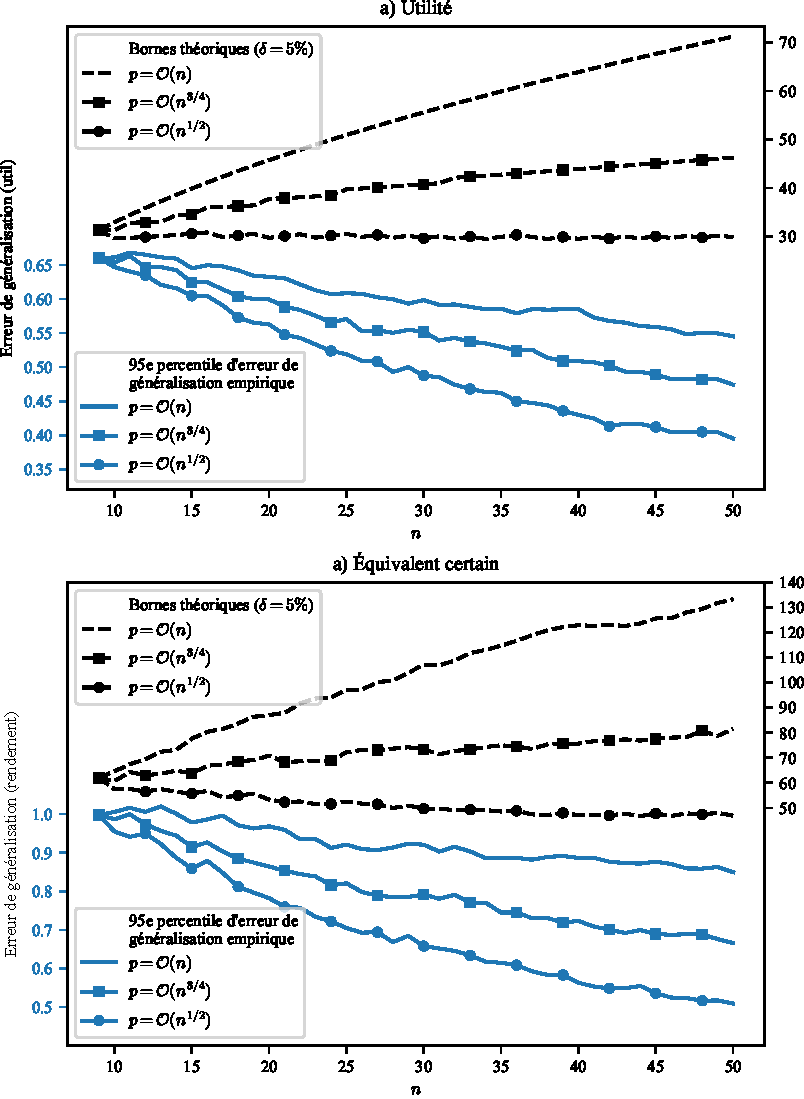
\includegraphics[width=\textwidth]{../experiments/fig/bound_npgenu.pdf}
  \caption[Erreur de généralisation -- Régimes $p=\bigO(n^{1/2}),\bigO(n^{3/4}),\bigO(n)$]
  {Progression du 95\ieme
    percentile d'erreur de généralisation et des garanties théorique en fonction de $n$,
    selon le régime de $p$. Une forte disparité entre la courbe des garanties théoriques
    et celle de l'erreur empirique est observée. Les courbes théoriques suggérant une
    progression de l'erreur $\bigO(p/n^{1/2})$, on se serait attendu à une amplification
    de l'erreur dès que $p$ domine $n^{1/2}$, \ie\ si $p=\omega(n^{1/2})$. Pourtant, cette
    figure indique que même si $p$ est de l'ordre de $n$, \ie\ $p = \bigO(n)$, l'erreur de
    généralisation empirique décroit tout de même.  }
  \label{fig_bound_npgenu}
\end{figure}

\begin{figure}[h!]
  \centering
  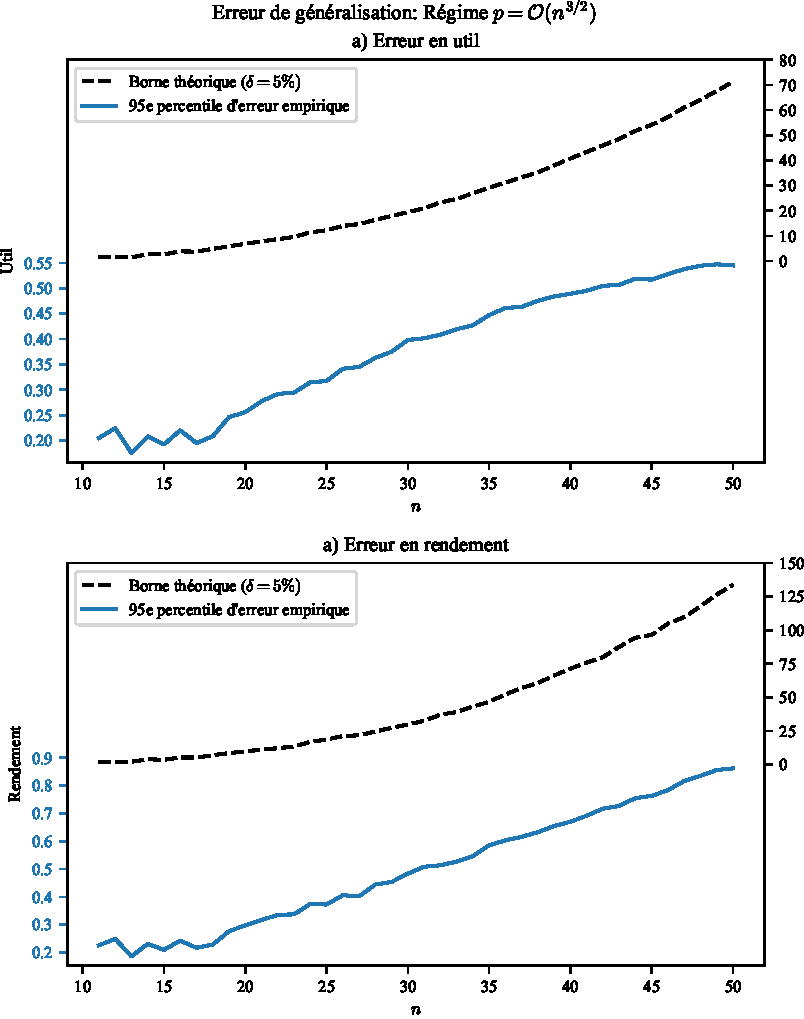
\includegraphics[width=\textwidth]{../experiments/fig/bound_np_np32.pdf}
  \caption[Erreur de généralisation -- Régime $p=\bigO(n^{3/2})$]{Progression du 95\ieme
    percentile de l'erreur de généralisation et de sa borne théorique $(\delta = 5\%)$ en
    fonction de la taille de l'échantillonage $n$. La relation entre $n$ et $p$ est donnée
    par la partie entière de $p = 0.0016n^{3/2}$. On observe bien une croissance de
    l'erreur de généralisation, cependant il serait trompeur de comparer ce résultat à
    celui présenté à la Figure \ref{fig_bound_npgenu} puisque le nombre $p$ de variables
    de marché est initialement beaucoup moins élevé dans ce cas-ci.}
  \label{fig_np_np32}
\end{figure}

\begin{figure}[h!]
  \centering
  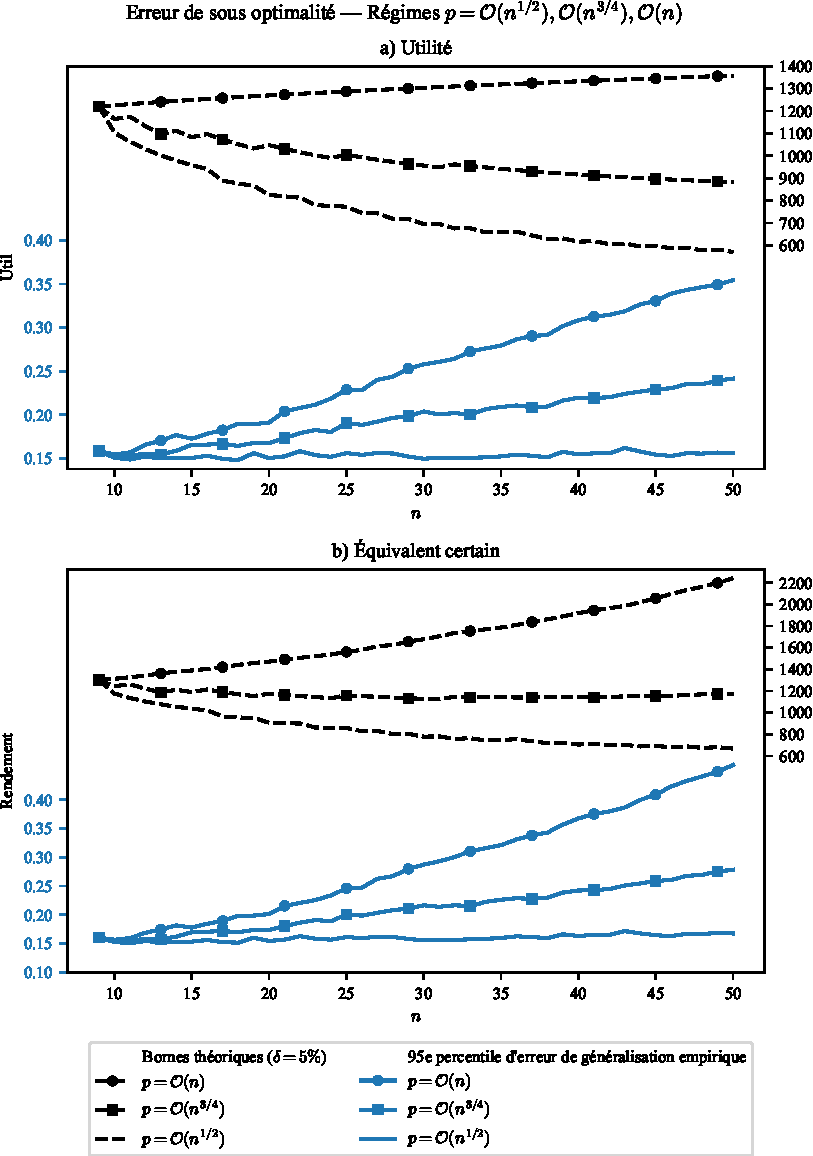
\includegraphics[width=\textwidth]{../experiments/fig/bound_test.pdf}
  \caption[Erreur de sous optimalité -- Régimes $p=\bigO(n^{1/2}),\bigO(n^{3/4}),\bigO(n)$]
  {Progression du 95\ieme percentile de l'erreur de sous optimalité et de sa garantie
    théorique $(\delta=5\%)$ selon les trois régimes à l'étude,
    $p=\bigO(n^{1/2}),p=\bigO(n^{3/4})$ et $p=\bigO(n)$. L'ordre $\bigO(p/\sqrt{n})$ de la
    borne semble ici respecté, puisque l'erreur de sous optimalité demeure constante dans
    le cas $p=\bigO(\sqrt{n})$, alors qu'elle augmente dans les deux autres
    cas. Cependant, les courbes théoriques décroissent, excepté lorsque $p=\bigO(n)$!}
  \label{fig_bound_npgsou}
\end{figure}

\clearpage

\subsection{Conclusion}

Cette section a permis d'illustrer le comportement des erreurs de généralisation et de
sous optimalité dans un cas relativement simple, où l'algorithme de décision ne disposait
que d'un noyau linéaire et où les variables de marché et le rendement étaient toutes
distribuées selon une loi Rademacher, liées les unes autres par une copule gaussienne.

Il a pu être établi assez clairement que pour un nombre constant de variables de marché,
l'erreur décroît bien à un rythme $\bigO(1/\sqrt{n})$, ce qui d'une certaine façon est
sans surprise au su du théorème limite centrale ou de la théorie de la programmation
stochastique (voir \cite{shapiro2009lectures}).

Les choses se compliquent sensiblement lorsqu'on fait intervenir un nombre croissant de
variables de marché. Néanmoins, avec $n$ constant, les expériences menées plus haut ont
permis de constater que l'ordre des deux types d'erreur est probablement $\bigO(p)$, bien
que ce régime puisse mettre du temps à apparaître et qu'il serait en fait plus précis de
parler d'un régime $\bigO(p) + \bigO(\sqrt{p})$.

La théorie par contre ne permet pas d'expliquer les courbes d'erreur de généralisation
observées dans des régimes dynamiques où $p=\bigO(n^k)$, où, pour $k\leq1$, celles-ci étaient
toutes décroissantes alors qu'elles auraient dû être croissantes. Ceci dit, l'étude faite
sur l'erreur de sous optimalité viendrait supporter l'idée que sa progression serait bien
de $\bigO(p/\sqrt{n})$. 




%%% Local Variables:
%%% mode: latex
%%% TeX-master: "memoire"
%%% End:


\newpage\section{Conclusion}

SVM multiclasse

Time series et learning


%%% Local Variables:
%%% mode: latex
%%% TeX-master: "main_conclusion"
%%% End:


\newpage\bibliography{../biblio}


\end{document}
%%% Local Variables:
%%% mode: latex
%%% TeX-master: t
%%% End:
